\documentclass[14pt]{beamer}
%\documentclass[handout]{beamer} %Makes Handouts
\usetheme{Singapore} %Gray with fade at top
\useoutertheme[subsection=false]{miniframes} %Supppress subsection in header
\useinnertheme{rectangles} %Itemize/Enumerate boxes
\usecolortheme{seagull} %Color theme
\usecolortheme{rose} %Inner color theme

\definecolor{light-gray}{gray}{0.75}
\definecolor{dark-gray}{gray}{0.55}
\setbeamercolor{item}{fg=light-gray}
\setbeamercolor{enumerate item}{fg=dark-gray}

\setbeamertemplate{navigation symbols}{}
\setbeamertemplate{mini frames}{}
%\setbeamercovered{dynamics}
\setbeamerfont*{title}{size=\Large,series=\bfseries}
\setbeamerfont{footnote}{size=\tiny}

%\setbeameroption{notes on second screen} %Dual-Screen Notes
%\setbeameroption{show only notes} %Notes Output

\setbeamertemplate{frametitle}{\vspace{.5em}\bfseries\insertframetitle}
\newcommand{\heading}[1]{\noindent \textbf{#1}\\ \vspace{1em}}
\newcommand{\questions}{\frame{\vspace{4em}\centering{\Large Questions?}}}
\newcommand{\StataActivity}[1]{\frame{\vspace{4em}\centering{\Large Let's work in Stata!\\ \vspace{1em} {(#1)}}}}


\usepackage{bbding,color,multirow,times,ccaption,tabularx,graphicx,verbatim,booktabs}
\usepackage{colortbl} %Table overlays
\usepackage[english]{babel}
\usepackage[latin1]{inputenc}
\usepackage[T1]{fontenc}
\usepackage{lmodern}
\usepackage{alltt}

\usepackage{tikz}
\usetikzlibrary{shapes,arrows,decorations.pathreplacing,calc}


\author[]{Thomas J. Leeper}
\institute{
  Government Department\\London School of Economics and Political Science
}


\title{Session I\\Survey Experiments in Context}

% ### Monday 30 January - *Morning*
% 
%  - Introduction to surveys, experiments, and the survey-experiment nexus
%  - History of survey experimentation
%  - Scientific and statistical logic of survey experiments
% 
% ### Monday 30 January - *Afternoon*
% 
%  - Translating theories into experimental designs
%  - Common survey experimental paradigms
%  - Discussion of applied examples

\date[]{30 January 2017}

\begin{document}

\frame{\titlepage}


\frame{

\frametitle{Activity!}

\only<2-4,6>{
\begin{enumerate}
\item<2-4,6> Ask you to guess a number
\item<3-4,6> Number off 1 and 2 across the room
\item<4,6> Group 2, close your eyes
\item<6> Group 1, close your eyes
\end{enumerate}
}

\Large
\only<5>{\textit{Group 1}\\ Think about whether the population of Chicago is more or less than 500,000 people. What do you think the population of Chicago is?}
\only<7>{\textit{Group 2}\\ Think about whether the population of Chicago is more or less than 10,000,000 people. What do you think the population of Chicago is?}

}
\frame{}

\frame{

\frametitle{Enter your data}

\begin{itemize}\itemsep1em
\item Go here: \url{http://bit.ly/297vEdd}
\item Enter your guess and your group number
\end{itemize}

%http://goo.gl/forms/xDW4FLm9pau0O8zz2

}


\frame{

\frametitle{Results}

\begin{itemize}\itemsep1em
\item True population: 2.79 million
\item<2-> What did you guess? \href{https://docs.google.com/spreadsheets/d/1SKWljS1EeNkAV5V0NZUwrKOu3LQFILVMB37xfTxyrPM/edit?usp=sharing}{(See Responses)}
\item<3-> What's going on here?
	\begin{itemize}
	\item An experiment!
	\item Demonstrates ``anchoring'' heuristic
	\end{itemize}
\item<4-> Experiments are easy to analyze, but only if designed and implemented well
\end{itemize}

}

\frame{\tableofcontents[subsubsectionstyle=hide]}

\frame{
\frametitle{Who am I?}

\small

\begin{itemize}\itemsep0.25em

\item Thomas Leeper

\item Assistant Professor in Political Behaviour at London School of Economics

\begin{itemize}
\item 2013--15: Aarhus University (Denmark)
\item 2008--12: PhD from Northwestern University (Chicago, USA)
\item Birth--2008: Minnesota, USA
\end{itemize}

\item Interested in public opinion and political psychology

\item Email: \href{mailto:t.leeper@lse.ac.uk}{t.leeper@lse.ac.uk}

\end{itemize}

}


\frame{

\frametitle{Who are you?}

\begin{itemize}\itemsep1em

\item Where are you from?

\item Have you designed a survey and/or experiment before?

\item What do you hope to learn from the course?

\end{itemize}

}



\frame{

\frametitle{Quick Survey}

\begin{enumerate}\itemsep0.5em
\item<2-> How many of you have worked with survey data before?
\item<3-> Of those, how many of you have \textit{performed} a survey before?
\item<4-> How many of you have worked with experimental data before?
\item<5-> Of those, how many of you have \textit{performed} an experiment before?
\end{enumerate}

}


\frame{

\frametitle{Course Materials}

\begin{center}
All material for the course is available at:\\

\vspace{1em}

\url{http://www.thomasleeper.com/surveyexpcourse/}
\end{center}

}

\frame{

\frametitle{Learning Outcomes}

\small

By the end of the day, you should be able to\dots

\begin{enumerate}
\item<2-> Explain how to analyze experiments quantitatively.
\item<3-> Explain how to design experiments that speak to relevant research questions and theories.
\item<4-> Evaluate the uses and limitations of several common survey experimental paradigms.
\item<5-> Identify practical issues that arise in the implementation of experiments and evaluate how to anticipate and respond to them.
\end{enumerate}

}




\section[History]{History of Experimentation}
\frame{\tableofcontents[currentsection,subsubsectionstyle=hide]}

\frame{

\frametitle{Experiments: Definition}

Oxford English Dictionary defines ``experiment'' as:

\begin{enumerate}
\item A scientific procedure undertaken to make a discovery, test a hypothesis, or demonstrate a known fact
\item A course of action tentatively adopted without being sure of the outcome
\end{enumerate}
}

\frame{

\frametitle{Experiments: History}

\begin{itemize}\itemsep0.75em
\item ``Experiments'' have a very long history

\item Major advances in design and analysis of experiments based on agricultural and later biostatistical research in the 19th century (Fisher, Neyman, Pearson, etc.)

\item First randomized, controlled trial (RCT) by Peirce and Jastrow in 1884

	\begin{itemize}
	\item<2-> First experiment by Gosnell (1924)
	\item<2-> Gerber and Green (2000) first major \textit{field} experiment
	\end{itemize}

\end{itemize}

}


\frame{
\centering
What distinguishes a \textit{survey} experiment from any other experiment?
}


\frame{

\begin{enumerate}\itemsep1em
\item Field Experiments
\item Laboratory Experiments
\item Survey Experiments
\end{enumerate}

Difference is only about \textit{setting} and \textit{mode}.\\

\only<2->{Logic and methods of analysis are the same!}

}






\frame{

\frametitle{Survey-Experiments}

\small

\begin{itemize}
\item Rise of surveys in the behavioral revolution
	\begin{itemize}
	\item Paper-and-pencil mode limited experimentation
	\item Limited use of ``split ballots''
	\end{itemize}
\item<2-> 1983: Merrill Shanks and the Berkeley Survey Research Center develop \textbf{CATI}
\item<3-> Mid-1980s: Paul Sniderman \& Tom Piazza performed the first survey experiment\only<3->{\footnote{Sniderman, Paul M., and Thomas Piazza. 1993. \textit{The Scar of Race}. Cambridge, MA: Harvard University Press.}}
	\begin{itemize}\footnotesize
	\item Then: the ``first multi-investigator''
	\item Later: Skip Lupia and Diana Mutz created TESS
	\end{itemize}
\end{itemize}

}



\frame{
\frametitle{{\large \textit{Survey}-experiments, specifically}}

\small

\begin{itemize}
\item<2-> A survey experiment is just an experiment that occurs in a survey context
	\begin{itemize}
	\item As opposed to in the field or in a laboratory
	\end{itemize}
\item<3-> Properties:
	\begin{itemize}
	\item Sample is representative of population in every respect (in expectation)
	\item Sample Average Treatment Effect (SATE) is the average of the sample's individual-level treatment effects
	\item SATE is unbiased estimate of PATE
	\end{itemize}
\item<4-> Sometimes a distinction is made between survey and online experiments
\end{itemize}
}


\frame{

\frametitle{TESS}

\small

\begin{itemize}
\item Time-Sharing Experiments for the Social Sciences
\item Multi-disciplinary initiative that provides infrastructure for survey experiments on nationally representative samples of the United States population
\item Funded by the U.S. National Science Foundation
\item Anyone anywhere in the world can apply\footnote{See also: \href{https://www.lissdata.nl/lissdata/}{LISS}, \href{http://www.uib.no/en/citizen}{Bergen's Citizen Panel}, \href{http://lore.gu.se/surveys/citizen}{Gothenburg's Citizen Panel}}
\end{itemize}

}

\frame{

\frametitle{TESS-like Projects}

There are some TESS-like initiatives outside the United States:

\begin{itemize}\itemsep1em
\item Netherlands: \href{https://www.lissdata.nl/lissdata/}{LISS}
\item Norway: \href{http://www.uib.no/en/citizen}{Bergen's Citizen Panel}
\item Sweden: \href{http://lore.gu.se/surveys/citizen}{Gothenburg's Citizen Panel}
\end{itemize}

}




\frame{

\frametitle{{\normalsize TESS has ``Open Protocols''}}

Protocol is the complete planning document for how to design, implement, and analyze an experiment.\footnote{Thomas J. Leeper. 2011. ``The Use of Protocol in the Design and Reporting of Experiments.'' \textit{The Experimental Political Scientist}.}

\small

\begin{enumerate}\itemsep-0.2em
\item Theory/hypotheses
\item Instrumentation
	\begin{itemize}
	\item Manipulation(s)
	\item Outcome(s)
	\item Covariate(s)
	\item Manipulation check(s)
	\end{itemize}
\item Sampling
\item Implementation
\item Analysis
\end{enumerate}
}

\frame{

\frametitle{Why bother writing a protocol?}

\begin{itemize}\itemsep0.5em
\item<2-> Be clear to yourself what you're trying to do before you do it
\item<3-> Assess the literature for best practices
\item<4-> Highlight areas in need of pilot testing
\item<5-> Economize questionnaire development
\item<6-> Study preregistration
\end{itemize}

}

\questions



\section[Logic]{Logic and Analysis}
\frame{\tableofcontents[currentsection,subsubsectionstyle=hide]}


\frame{
	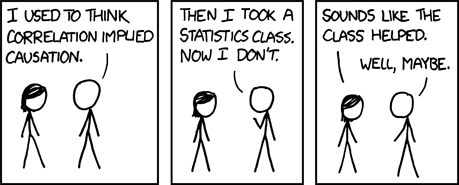
\includegraphics[width=\textwidth]{images/xkcdcorrelation.png}
}


\frame{

\frametitle{Addressing Confounding}

In observational research\dots

\begin{enumerate}\itemsep0.5em
\item<2-> Correlate a ``putative'' cause ($X$) and an outcome ($Y$)
\item<3-> Identify all possible confounds (\textbf{Z})
\item<4-> ``Condition'' on all possibl econfounds
	\begin{itemize}
	\item Calculate correlation between $X$ and $Y$ at each combination of levels of \textbf{Z}
	\end{itemize}
\item<5-> Basically: $Y = \beta_0 + \beta_1 X + \beta Z + \epsilon $
\end{enumerate}

}


\begin{frame}
\begin{center}
\begin{tikzpicture}[>=latex',circ/.style={draw, shape=circle, node distance=5cm, line width=1.5pt}]
    \draw (0,0) node[left] (X) {\textcolor<2->{red}{Smoking}};
    \draw[->] (X) -- (5,0) node[right] (Y) {Cancer};
    \draw[->] (-3,3) node[above] (Z) {Sex} -- (X);
    \draw[->] (Z) -- (Y);
    \draw[->] (5,2) node[above] (A) {Environment} -- (Y);
    \draw[->] (4,-3) node[below, text width=3cm, align=center] (E) {Genetic\\Predisposition} -- (Y);
    \draw[->] (-2, -2) node[below, text width=2.5cm, align=center] (W) {Parental\\Smoking} -- (X);
    \draw[->] (W) -- (Y);
    \draw<2->[->, dashed, very thick] (E) -- (X);
\end{tikzpicture}
\end{center}
\end{frame}




\frame{

\frametitle{Experiments are different}

\begin{enumerate}\itemsep0.75em
\item<2-> Draw causal inferences through \textit{design} not \textit{analysis}
\item<3-> Randomization breaks selection bias
\item<4-> We don't need to ``control'' for anything
\item<5-> We see ``causal effects'' in the comparison of experimental groups
\end{enumerate}

}


% Mill's method of difference
\frame{
\frametitle{{\normalsize Mill's Method of Difference}}

\small

If an instance in which the phenomenon under investigation occurs, and an instance in which it does not occur, \textbf<2->{have every circumstance save one in common}, that one occurring only in the former; \textbf<2->{the circumstance in which alone the two instances differ, is the} effect, or \textbf<2->{cause}, or an necessary part of the cause, \textbf<2->{of the phenomenon}.
}



\frame{

\frametitle{Definitions}

\only<2>{\textbf{Unit}: A physical object at a particular point in time}

\only<3>{\textbf{Treatment}: An intervention, whose effect(s) we wish to assess relative to some other (non-)intervention}

\only<4>{
\textbf{Potential outcomes}: The outcome for each unit that we would observe if that unit received each treatment
\begin{itemize}
\item Multiple potential outcomes for each unit, but we only observe one of them
\end{itemize}
}

\only<5>{\textbf{Causal effect}: The comparisons between the unit-level potential outcomes under each intervention}

}




% Individual-level effects versus ATEs


\frame{
	\frametitle{The Experimental Ideal}
	\small
	A randomized experiment, or randomized control trial is:
 		\begin{quote}\small
 			The observation of units after, and possibly before, a randomly assigned intervention in a controlled setting, which tests one or more precise causal expectations
 		\end{quote}
 	This is Holland's ``statistical solution'' to the fundamental problem of causal inference
}


\frame{
\frametitle{Two solutions!\footnote{From Holland}}

\begin{enumerate}\itemsep1em
\item Scientific Solution
	\begin{itemize}
	\item All units are identical
	\item Each can provide a perfect counterfactual
	\item Common in, e.g., agriculture, biology
	\end{itemize}
\item<2-> Statistical Solution
	\begin{itemize}
	\item Units are not identical
	\item Random exposure to a potential cause
	\item Effects measured on average across units
	\item Known as the ``Experimental ideal''
	\end{itemize}
\end{enumerate}

}



\frame{
\frametitle{The Experimental Ideal}
\begin{itemize}\itemsep0.5em
\item It solves both the temporal ordering and confounding problems of observational causal inference
	\begin{itemize}
   		\item Treatment ($X$) is applied by the researcher before outcome ($Y$)
   		\item Randomization means there are no confounding ($Z$) variables
	\end{itemize}
\item<2-> Thus experiments are a ``gold standard'' of causal inference
\item<3-> Basically: $Y = \beta_0 + \beta_1 X + \epsilon $
\end{itemize}
}


\frame{

\frametitle{Neyman--Rubin Potential Outcomes Framework}

If we are interested in some outcome $Y$, then for every unit $i$, there are numerous ``potential outcomes'' $Y*$ only one of which is visible in a given reality. Comparisons of (partially unobservable) potential outcomes indicate causality.

}

\frame{

\frametitle{Neyman--Rubin Potential Outcomes Framework}

Concisely, we typically discuss two potential outcomes:

\begin{itemize}\small
\item $Y_{0i}$, the \textit{potential} outcome \textit{realized} if $X_i = 0$ (b/c $D_i = 0$, assigned to control)
\item $Y_{1i}$, the \textit{potential} outcome \textit{realized} if $X_i = 1$ (b/c $D_i = 1$, assigned to treatment)
\end{itemize}

}


\frame{

\frametitle{Historical Aside}

\small

\begin{itemize}
\item The history of the potential outcomes framework is contested
\item Most people attribute it to Donald Rubin
\item Paul Holland was the first to link to the philosophical discussions of causality
\item Donald Rubin attributes this to Jerzy Neyman (1923)
\item James Heckman denies all of this and attributes it Andrew Roy (1951)
\end{itemize}
}







% design-based experimental inference
\frame{
	\frametitle{Experimental Inference I}
	\small
	\begin{itemize}\itemsep0.5em
    	\item<1-> Each unit has multiple \textit{potential} outcomes, but we only observe one of them, randomly
    	\item<2-> In this sense, we are sampling potential outcomes from each unit's population of potential outcomes
		\only<2->{
			\begin{center}
			\begin{tabular}{ccccc}
			unit & low & high & \onslide<3->{control} & \onslide<4->{etc.} \\ \midrule
			1 & ? & ? & \onslide<3->{?} & \onslide<4->{\dots} \\
			2 & ? & ? & \onslide<3->{?} & \onslide<4->{\dots} \\
			3 & ? & ? & \onslide<3->{?} & \onslide<4->{\dots} \\
			4 & ? & ? & \onslide<3->{?} & \onslide<4->{\dots} \\ \bottomrule
			\end{tabular}
			\end{center}
		}
	\end{itemize}
}

\frame{
	\frametitle{Experimental Inference II}
	\small
	\begin{itemize}\itemsep0.5em
    	\item<1-> We cannot see individual-level causal effects
    	\item<2-> We can see \textit{average causal effects}
    		\begin{itemize}
        		\item<2-> Ex.: Average difference in cancer between those who do and do not smoke
    		\end{itemize}
    	\item<3-> We want to know: $TE_i = Y_{1i} - Y_{0i}$
	\end{itemize}
}

\frame{
	\frametitle{Experimental Inference III}
	\small
	\begin{itemize}\itemsep0.5em
		\item<1-> We want to know: $TE_i = Y_{1i} - Y_{0i}$ for every $i$ in the population
		\item<2-> We can average: $E[TE_i] = E[Y_{1i} - Y_{0i}] = E[Y_{1i}] - E[Y_{0i}]$
		\item<3-> But we still only see one potential outcome for each unit:\\ \vspace{1em}
    		$ATE_{naive} = E[Y_{1i} | X = 1] - E[Y_{0i} | X = 0]$
    	\item<4-> Is this what we want to know?
	\end{itemize}
}


\frame{
	\frametitle{Experimental Inference IV}
	\small
	\begin{itemize}\itemsep0.5em
	\item What we want and what we have:
		\begin{align}
		ATE & = E[Y_{1i}] - E[Y_{0i}] \\[1em]
		ATE_{naive} & = E[Y_{1i} | X = 1] - E[Y_{0i} | X = 0]
		\end{align}		
	\item<2-> Are the following statements true?\\
  		\begin{itemize}\itemsep0.5em
      		\item<2-> $E[Y_{1i}] = E[Y_{1i} | X = 1]$
      		\item<2-> $E[Y_{0i}] = E[Y_{0i} | X = 0]$
  		\end{itemize}
  	\item<3-> Not in general!
  	\end{itemize}
}

\frame{
	\frametitle{Experimental Inference V}
	\small
	\begin{itemize}\itemsep0.5em
    	\item Only true when both of the following hold:
    	\begin{align}
    	E[Y_{1i}] = E[Y_{1i} | X = 1] = E[Y_{1i} | X = 0]\\
    	E[Y_{0i}] = E[Y_{0i} | X = 1] = E[Y_{0i} | X = 0]
    	\end{align}
    	\item In that case, potential outcomes are \textit{independent} of treatment assignment
		\item If true (e.g., due to randomization of $X$), then:
    	\begin{align*}
    	ATE_{naive} & = E[Y_{1i} | X = 1] - E[Y_{0i} | X = 0] \tag{5}\\
    	& = E[Y_{1i}] - E[Y_{0i}]\\
    	& = ATE
    	\end{align*}
	\end{itemize}
}

\frame{
	\frametitle{Experimental Inference VI}

	\normalsize
	\begin{itemize}\itemsep0.5em
    	\item This holds in experiments because of a \textit{physical process of randomization}\footnote{Random means ``known probability of treatment'' not ``haphazard''.}
   		\item<2-> Units differ only in side of coin that was up
	   		\begin{itemize}\footnotesize
	   		\item $X_i = 1$ only because $D_i = 1$
	   		\end{itemize}
	   	\item<3-> Implications:
		   	\begin{itemize}
		   	\item Covariate balance
		   	\item Potential outcomes balanced and independent of treatment assignment
		   	\item No confounding (selection bias)
		   	\end{itemize}
	\end{itemize}
}




\begin{frame}
\small 
\begin{center}
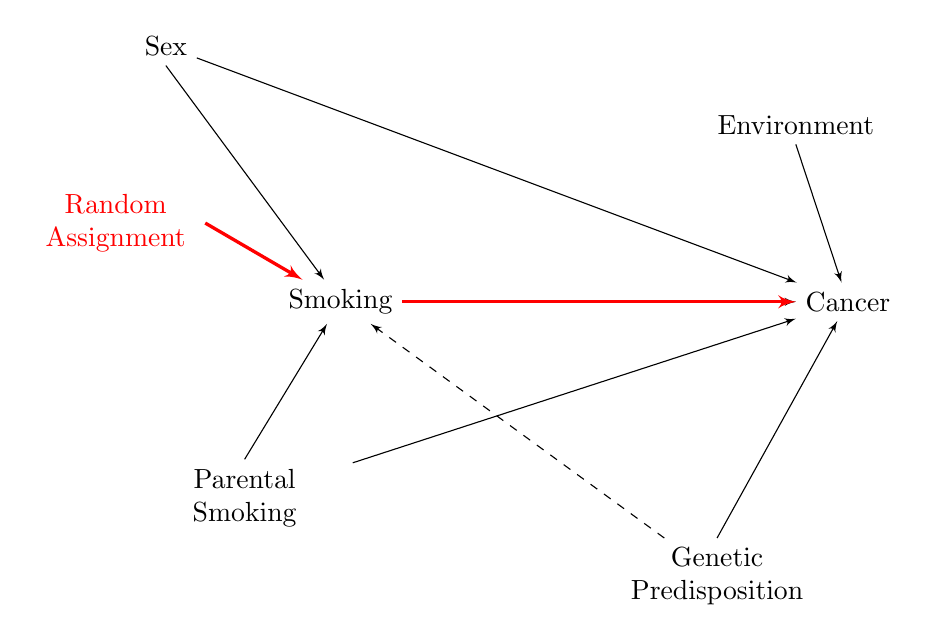
\begin{tikzpicture}[>=latex',circ/.style={draw, shape=circle, node distance=5cm, line width=1.5pt}]
    \draw[->] (0,0) node[left] (X) {Smoking} -- (5,0) node[right] (Y) {Cancer};
    \draw[->] (-3,3) node[above] (Z) {Sex} -- (X);
    \draw[->] (Z) -- (Y);
    \draw[->] (5,2) node[above] (A) {Environment} -- (Y);
    \draw[->] (4,-3) node[below, text width=3cm, align=center] (E) {Genetic\\Predisposition} -- (Y);
    \draw[->] (-2, -2) node[below, text width=2.5cm, align=center] (W) {Parental\\Smoking} -- (X);
    \draw[->] (W) -- (Y);
    \draw[->, dashed] (E) -- (X);
    
    \draw<2->[->, very thick, color=red] (-2.5,1) node[left, color=red, text width=2cm, align=center] (Tr) {Random\\Assignment} -- (X);
    \draw<2->[->, very thick, color=red] (X) -- (Y);
\end{tikzpicture}
\end{center}
\end{frame}

\questions



\frame{

\large
\centering
Does randomization \textit{guarantee balance}? Does it work every time?

\only<2->{What happens if there is imbalance? How would we know?}
}


\frame{

\frametitle{Balance Testing I}

\begin{itemize}\itemsep0.5em
\item Analysis of experiments assumes that randomization produces covariate balance
\item<2-> But this is only true \textit{in expectation}
\item<3-> If we find covariate imbalance, we can:
	\begin{itemize}
	\item Ignore it
	\item Condition on imbalanced covariates
	\end{itemize}
\end{itemize}

}

\frame{

\frametitle{Balance Testing II}

There are three basic ways to detect covariate imbalance:

\begin{enumerate}\itemsep1em
\item Regressing treatment assignment on covariates
\item Conducting t-tests for each covariate across experimental groups
\item Examining covariate means visually
\end{enumerate}

}

\StataActivity{Balance testing!}



\frame{}

\frame{

\large\centering
The other solution --- if possible --- is to \textit{block randomize}.

}


\frame{

\frametitle{Block Randomization I}

{\small \textbf{Stratification:Sampling::Blocking:Experiments}}

\small

\begin{itemize}\itemsep0.5em
\item<2-> Basic idea: randomization occurs within strata defined before treatment assignment
\item<3-> CATE is estimate for each stratum; aggregated to SATE
\item<4-> Why?
	\begin{itemize}
	\item Eliminate chance imbalances
	\item Optimized for estimating CATEs
	\item More precise SATE estimate
	\end{itemize}
\end{itemize}

}

\begin{frame}[fragile]

\begin{center}
\begin{tabular}{lcccccccc}
Exp. & \multicolumn{4}{c}{Control} & \multicolumn{4}{c}{Treatment} \\ \midrule
1 & M & M & M & M & F & F & F & F \\
2 & M & M & M & F & M & F & F & F \\
3 & M & M & F & F & M & M & F & F \\
4 & M & F & F & F & M & M & M & F \\
5 & F & F & F & F & M & M & M & M \\ \bottomrule
\end{tabular}
\end{center}

\end{frame}

\frame{

\begin{center}

\begin{tabular}{rrrr}
Obs. & $X_{1i}$ & $X_{2i}$ & $D_i$ \\ \midrule
1 & Male & Old & 0 \\
2 & Male & Old & 1 \\  \midrule
3 & Male & Young & 1 \\
4 & Male & Young & 0 \\ \midrule
5 & Female & Old & 1 \\
6 & Female & Old & 0 \\ \midrule
7 & Female & Young & 0 \\
8 & Female & Young & 1 \\ \bottomrule
\end{tabular}
\end{center}

}

\frame[label=blocking2]{

\frametitle{Block Randomization II}

\begin{itemize}
\item Blocking ensures ignorability of all covariates used to construct the blocks
\item Incorporates covariates explicitly into the \textit{design}
\item<2-> When is blocking \textit{statistically} useful?
	\begin{itemize}
	\item<3-> If those covariates affect values of potential outcomes, blocking reduces the variance of the SATE
	\item<4-> Most valuable in small samples
	\item<5-> Not valuable if all blocks have similar potential outcomes
	\end{itemize}
\end{itemize}

}



\frame{

\frametitle{Statistical Properties I}

\small

Complete randomization:\\
$$SATE = \frac{1}{n_1}\sum Y_{1i} - \frac{1}{n_0}\sum Y_{0i}$$

\vspace{2em}

Block randomization:\\
$$SATE_{blocked} = \sum_{1}^{J} \left( \dfrac{n_j}{n} \right)  (\widehat{CATE}_j)$$

}


\frame{

\begin{center}

\begin{tabular}{rrrrrr}
Obs. & $X_{1i}$ & $X_{2i}$ & $D_i$ & $Y_i$ & CATE \\ \midrule
1 & Male & Old & 0 & 5 & \multirow{2}{*}{\onslide<2->{5}} \\
2 & Male & Old & 1 & 10 \\  \midrule
3 & Male & Young & 1 & 4 & \multirow{2}{*}{\onslide<3->{3}} \\
4 & Male & Young & 0 & 1 \\ \midrule
5 & Female & Old & 1 & 6 & \multirow{2}{*}{\onslide<4->{4}} \\
6 & Female & Old & 0 & 2 \\ \midrule
7 & Female & Young & 0 & 6 & \multirow{2}{*}{\onslide<5->{3}} \\
8 & Female & Young & 1 & 9 \\ \bottomrule
\end{tabular}
\end{center}

}

\frame{

\frametitle{SATE Estimation}

\begin{align*}
SATE &= \left(\dfrac{2}{8}*5\right) + \left(\dfrac{2}{8}*3\right) + \left(\dfrac{2}{8}*4\right) + \left(\dfrac{2}{8}*3\right) \\ \vspace{1em}
&= 3.75
\end{align*}

\onslide<2->{The blocked and unblocked estimates are the same here because $Pr(Treatment)$ is constant across blocks and blocks are all the same size.}

}

\frame{

\frametitle{SATE Estimation}

\small

\begin{itemize}
\item We can use weighted regression to estimate this in an OLS framework
\item Weights are the inverse prob. of being treated w/in block
\begin{itemize}
\item Pr(Treated) by block: $p_{ij} = Pr(D_i = 1 | J=j) $
\item Weight (Treated): $ w_{ij} = \dfrac{1}{p_{ij}} $
\item Weight (Control): $ w_{ij} = \dfrac{1}{1-p_{ij}} $
\end{itemize}
\end{itemize}

}


\frame{

\frametitle{Statistical Properties II}

\small

Complete randomization:\\
$$\widehat{SE}_{SATE} = \sqrt{\dfrac{\widehat{Var}(Y_0)}{n_0} + \dfrac{\widehat{Var}(Y_1)}{n_1}}$$

\vspace{1em}

Block randomization:\\
$$\widehat{SE}_{SATE_{blocked}} = \sqrt{\sum_{1}^{J} \left( \dfrac{n_j}{n} \right)^2  \widehat{Var}{(SATE_j)}}$$

\only<2->{When is the blocked design more efficient?}

}


\frame{

\frametitle{Practicalities}

\begin{itemize}\itemsep0.5em
\item Blocked randomization only works in exactly the same situations where stratified sampling works
	\begin{itemize}
	\item Need to observe covariates pre-treatment in order to block on them
	\item Work best in a panel context
	\end{itemize}
\item In a single cross-sectional design that might be challenging
	\begin{itemize}
	\item Some software can block ``on the fly''
	\end{itemize}
\end{itemize}


}

\questions

\frame{}



\frame{
\frametitle{Experimental Analysis}
\small
\begin{itemize}
\item The statistic of interest in an experiment is the \textit{sample average treatment effect} (SATE)
\item If our sample is \textit{representative}, then this provides an estimate of the population average treatment (PATE)
\item This boils down to being a mean-difference between two groups:
	\begin{equation}
	SATE = \frac{1}{n_1}\sum Y_{1i} - \frac{1}{n_0}\sum Y_{0i}
	\end{equation}
\item<2->The Neyman--Rubin logic only works for \textit{means}\footnote{But not medians, etc.}
\end{itemize}
}



\frame{

\frametitle{Computation of Effects}

\begin{itemize}\itemsep0.5em
\item In practice we often estimate SATE using t-tests, ANOVA, or OLS regression
\item These are all basically equivalent
\item<2-> Reasons to choose one procedure over another:
	\begin{itemize}
	\item<2-> Disciplinary norms
	\item<3-> Ease of interpretation
	\item<4-> Flexibility for >2 treatment conditions
	\end{itemize}
\end{itemize}



}

\frame[label=tidy]{

\frametitle{Experimental Data Tidying}

An experimental data structure looks like:

\small

\begin{center}
\begin{tabular}{ccc}
\texttt{unit} & \texttt{treatment} & \texttt{outcome} \\ \hline 
1 & 0 & 13 \\
2 & 0 & 6 \\
3 & 0 & 4 \\
4 & 0 & 5 \\
5 & 1 & 3 \\
6 & 1 & 1 \\
7 & 1 & 10 \\
8 & 1 & 9 \\ \hline
\end{tabular}
\end{center}

}

\frame{

\frametitle{Experimental Data Tidying}

Sometimes it looks like this instead, which is bad:

\small

\begin{center}
\begin{tabular}{cccc}
\texttt{unit} & \texttt{treatment} & \texttt{outcome0}  & \texttt{outcome1} \\ \hline 
1 & 0 & 13 & . \\
2 & 0 & 6 & . \\
3 & 0 & 4 & . \\
4 & 0 & 5 & . \\
5 & 1 & . & 3 \\
6 & 1 & . & 1 \\
7 & 1 & . & 10 \\
8 & 1 & . & 9 \\ \hline
\end{tabular}
\end{center}

}

\againframe{tidy}


\frame{

\frametitle{Experimental Data Tidying}

Sometimes it looks like this instead, which is even worse:

\small

\begin{center}
\begin{tabular}{cccc}
\texttt{unit} & \texttt{treatment} & \texttt{outcome0}  & \texttt{outcome1} \\ \hline 
1 & . & 13 & . \\
2 & . & 6 & . \\
3 & . & 4 & . \\
4 & . & 5 & . \\
5 & . & . & 3 \\
6 & . & . & 1 \\
7 & . & . & 10 \\
8 & . & . & 9 \\ \hline
\end{tabular}
\end{center}

}

\againframe{tidy}







\begin{frame}[fragile]

\frametitle{Computation of Effects in Stata}

Stata:\small
\begin{verbatim}
ttest outcome, by(treatment)
reg outcome i.treatment
\end{verbatim}

R:\small
\begin{verbatim}
t.test(outcome ~ treatment, data = data)
lm(outcome ~ factor(treatment), data = data)
\end{verbatim}

\end{frame}


\questions

\StataActivity{Basic analysis}











\frame{
\frametitle{SATE Variance Estimation}
	\small
\begin{itemize}\itemsep0.5em
\item We don't just care about the size of the SATE. We also want to know whether it is significantly different from zero (i.e., different from no effect/difference)
\item To know that, we need to estimate the \textit{variance} of the SATE
\item The variance is influenced by:
	\begin{itemize}
	\item Total sample size
	\item Variance of the outcome, $Y$
	\item Relative size of each treatment group
	\end{itemize}
\end{itemize}
}


\frame{
\frametitle{SATE Variance Estimation}
	\small
\begin{itemize}\itemsep0.5em
\item Formula for the variance of the SATE is:\\
$\widehat{Var}(SATE) = \dfrac{\widehat{Var}(Y_0)}{n_0} + \dfrac{\widehat{Var}(Y_1)}{n_1}$

	\begin{itemize}
	\item $\widehat{Var}(Y_0)$ is control group variance
	\item $\widehat{Var}(Y_1)$ is treatment group variance
	\end{itemize}

\item We often express this as the \textit{standard error} of the estimate:\\
$\widehat{SE}_{SATE} = \sqrt{\frac{\widehat{Var}(Y_0)}{n_0} + \frac{\widehat{Var}(Y_1)}{n_1}}$
\end{itemize}
}


\frame{

\frametitle{Intuition about Variance}

\begin{itemize}\itemsep0.5em
\item Bigger sample $\rightarrow$ smaller SEs
\item Smaller variance $\rightarrow$ smaller SEs
\item Efficient use of sample size:
	\begin{itemize}
	\item When treatment group variances equal, equal sample sizes are most efficient
	\item When variances differ, sample units are better allocated to the group with higher variance in \emph{Y}
	\end{itemize}
\end{itemize}

}


\frame{
	\frametitle{Important considerations}
	\begin{itemize}\itemsep0.5em
		\item Required sample size depends on $SATE$ and $Var(Y)$
		\item<2-> In large populations, population size is irrelevant
		\item<3-> In small populations, precision is influenced by the proportion of population sampled
		\item<4-> In anything other than an SRS, sample size calculation is more difficult
		\item<5-> Most research assumes SRS even though a more complex design is actually used
		\item<6-> Sample size needed to obtain a precise estimate of SATE is always going to be twice as large as needed to obtain an precise estimate of $\bar{Y}$
	\end{itemize}
}

\frame{
	\frametitle{Estimating sample size}
	What precision (margin of error) do we want?
	\begin{itemize}
		\item $p$ +/- 5 percentage points: $SE = 0.025$
			\begin{equation}
			n = \frac{0.25}{0.000625} = 400
			\end{equation}
		\item<2-> $p$ +/- 2 percentage points: $SE = 0.01$
			\begin{equation}
			n = \frac{0.25}{0.01^2} = \frac{0.25}{0.0001} = 2500
			\end{equation}
		\item<3-> $p$ +/- 0.5 percentage points: $SE = 0.0025$
			\begin{equation}
			n = \frac{0.25}{0.00000625} = 40,000
			\end{equation}
	\end{itemize}
}


\frame{

\frametitle{Statistical Power}

\begin{itemize}\itemsep0.5em
\item Power analysis to determine sample size
\item Type I and Type II Errors
	\begin{itemize}
	\item True positive rate is power
	\item False negative rate is the significance threshold ($\alpha$)
	\end{itemize}
\end{itemize}

\begin{tabular}{lrr}
\toprule
& $H_0$ True & $H_0$ False \\ \midrule
Reject $H_0$ & Type 1 Error & \textbf{True positive} \\
Accept $H_0$ & False negative & Type II error \\ \bottomrule
\end{tabular}

}


\frame{

\frametitle{Doing a Power Analysis}

\begin{itemize}
\item $\mu$, Treatment group mean outcomes
\item $N$, Sample size
\item $\sigma$, Outcome variance
\item $\alpha$ Statistical significance threshold
\item $\phi$, a sampling distribution
\end{itemize}

$Power = \phi\left( \frac{|\mu_1 - \mu_0|\sqrt{N}}{2\sigma} - \phi^{-1}\left( 1 - \frac{\alpha}{2} \right) \right)$

}



\frame{
\frametitle{Intuition about Power}

Minimum detectable effect is the smallest effect we could detect given sample size, ``true'' effect size, variance of outcome, power, and $\alpha$.\\

\vspace{0.5em}

In essence: some non-zero effect sizes are not detectable by a study of a given sample size.\footnote{Gelman, A. and Weakliem, D. 2009. ``Of Beauty, Sex and Power.'' \textit{American Scientist} 97(4): 310--16}

}


\frame{

\frametitle{Intuition about Power}

\begin{itemize}\itemsep0.5em
\item It can help to think in terms of ``standardized effect sizes''
\item Cohen's $d$:\\ $d = \frac{\bar{x}_1 - \bar{x}_0}{s}$, where
$s = \sqrt{\frac{(n_1 - 1)s_1^2 + (n_0 - 1)s_0^2}{n_1 + n_0 - 2}}$
\item Intuition: How large is the effect in standard deviations of the outcome?
	\begin{itemize}
	\item Know if effects are large or small
	\item Compare effects across studies
	\end{itemize}
\item Small: 0.2; Medium: 0.5; Large: 0.8
\end{itemize}

}

\StataActivity{Power Analysis}


\frame{
\frametitle{Intuition about Power}

\begin{center}
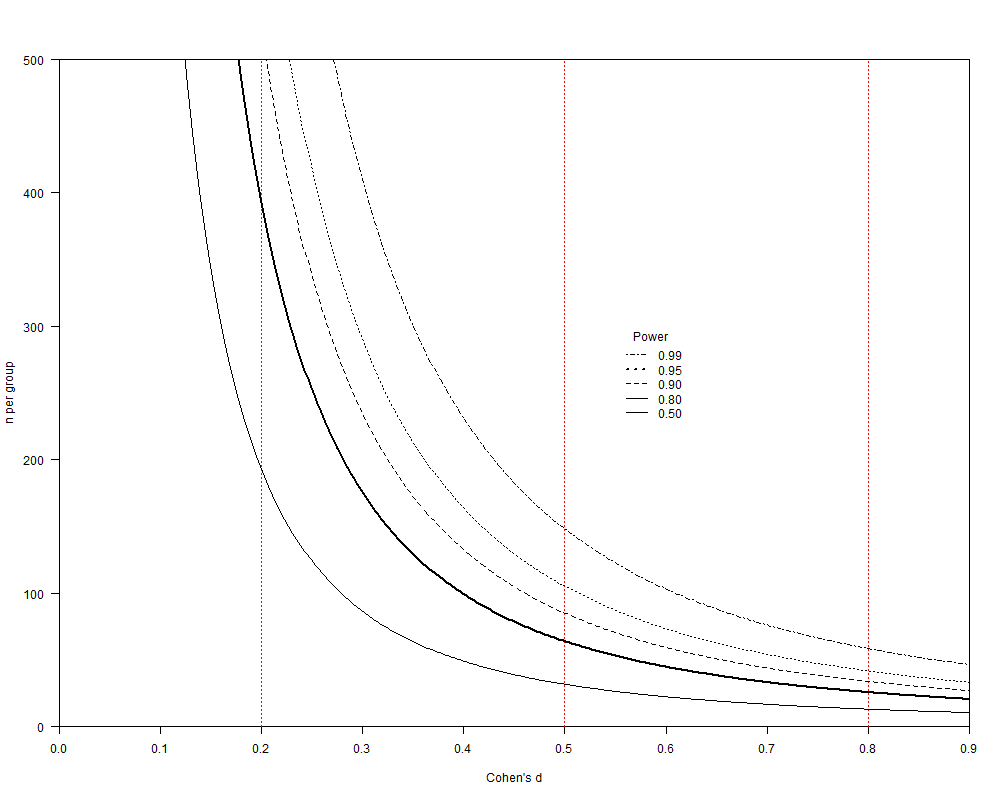
\includegraphics[height=0.8\textheight, trim = 0in 0in 0in 0.5in , clip]{images/power}
\end{center}

}








\frame{}


\section[Theory$\rightarrow$Design]{From Theory to Design}
\frame{\tableofcontents[currentsection,subsubsectionstyle=hide]}
% deriving hypotheses from theory and manipulations from hypotheses


\frame{

\frametitle{{\normalsize What kinds of questions can we answer with (survey) experiments?}}

\normalsize

\begin{itemize}\itemsep0.5em
\item<2-> Forward causal questions
	\begin{itemize}
	\item Can X cause Y?
	\item What effects does X have?
	\end{itemize}
\item<3-> Backward causal questions
	\begin{itemize}
	\item What causes Y?
	\item How much of Y is attributable to X?
	\end{itemize}
\item<4-> Even though answering ``forward'' causal question, we start with an outcome concept
\end{itemize}
}



\section[Principles]{Operationalization Principles}

\frame{

\frametitle{Hypothesis Testing}

\begin{itemize}\itemsep0.5em
\item From theory, we derive testable hypotheses
\begin{itemize}
\item Hypotheses are expectations about differences in outcomes across levels of a putatively causal variable
\item Hypothesis must be testable by an SATE
\end{itemize}
\item Manipulations are developed to create variation in that causal variable
\end{itemize}

}


\frame{

\frametitle{{\normalsize Example: News Framing}}

\small

\begin{itemize}
\item Theory: Presentation of news affects opinion
\item Hypotheses:
	\begin{itemize}\footnotesize
	\item News emphasizing free speech increases support for a hate group rally
	\item News emphasizing public safety decreases support for a hate group rally
	\end{itemize}
\item Manipulation:
	\begin{itemize}\footnotesize
	\item Control group: no information
	\item Free speech group: article emphasizing rights
	\item Public safety group: article emphasizing safety
	\end{itemize}
\end{itemize}

}




\frame{

\frametitle{{\normalsize Example: Partisan Identity}}

\small

\begin{itemize}
\item Theory: Strength of partisan identity affects tendency to accept party position
\item Hypotheses:
	\begin{itemize}\small
	\item Strong partisans are more likely to accept their party's position on an issue
	\end{itemize}
\item Manipulation:
	\begin{itemize}\small
	\item Control group: no manipulation
	\item ``Univalent'' condition
	\item ``Ambivalent'' condition
	\end{itemize}
\end{itemize}

}


\frame[label=ambivalentpartisan]{

\frametitle{\textbf{\only<1>{Univalent}\only<2>{Ambivalent}}}

These days, Democrats and Republicans differ from one another considerably. The two groups seem to be growing further and further apart, not only in terms of their opinions but also their lifestyles. Earlier in the survey, you said you tend to identify as a \textit{Democrat/ Republican}. Please take a few minutes to think about what you like about \textit{Democrats/ Republicans} compared to the \textit{Republicans/ Democrats}. Think of 2 to 3 things you especially like best about \textbf{\only<1>{your party}\only<2>{the other party}}. Then think of 2 to 3 things you especially dislike about \textbf{\only<2>{your party}\only<1>{the other party}}. Now please write those thoughts in the space below.

}



\frame{

\frametitle{Treatments Test Hypotheses!}

\begin{itemize}\itemsep0.5em
\item<2-> Derive experimental design from hypotheses
\item<3-> Experimental ``factors'' are expressions of hypotheses as randomized groups
\item<4-> What intervention each group receives depends on hypotheses
	\begin{itemize}
	\item presence/absence
	\item levels/doses
	\item qualitative variations
	\end{itemize}
\end{itemize}

}


\frame{

\frametitle{{\normalsize Ex.: Presence/Absence}}

\small

\begin{itemize}\itemsep0.5em
\item Theory: Negative campaigning reduces support for the party described negatively.
\item Hypothesis: Exposure to a negative advertisement criticizing a party reduces support for that party.
\item Manipulation:
	\begin{itemize}\small 
	\item Control group receives no advertisement. 
	\item Treatment group watches a video containing a negative ad describing a party.
	\end{itemize}
\end{itemize}

}


\frame{

\frametitle{{\normalsize Ex.: Levels/doses}}

\small

\begin{itemize}\itemsep-0.2em
\item Theory: Negative campaigning reduces support for the party described negatively.
\item Hypothesis: Exposure to higher levels of negative advertising criticizing a party reduces support for that party.
\item Manipulation:
	\begin{itemize}\footnotesize
	\item Control group receives no advertisement. 
	\item Treatment group 1 watches a video containing 1 negative ad describing a party.
	\item Treatment group 2 watches a video containing 2 negative ads describing a party.
	\item Treatment group 3 watches a video containing 3 negative ads describing a party.
	\item etc.
	\end{itemize}
\end{itemize}

}


\frame{

\frametitle{{\normalsize Ex.: Qualitative variation}}

\small

\begin{itemize}
\item Theory: Negative campaigning reduces support for the party described negatively.
\item Hypothesis: Exposure to a negative advertisement criticizing a party reduces support for that party, while a positive advertisement has no effect.
\item Manipulation:
	\begin{itemize}\footnotesize
	\item Control group receives no advertisement. 
	\item Negative treatment group watches a video containing a negative ad describing a party.
	\item Positive treatment group watches a video containing a positive ad describing a party.
	\end{itemize}
\end{itemize}

}

\questions


\frame{}



\frame{

\frametitle{Activity!}

\begin{itemize}\itemsep0.5em
\item How do we know if an experiment is any good?
\item Talk with a partner for about 3 minutes
\item Try to develop some criteria that allow you to evaluate ``what makes for a good experiment?'' 
\end{itemize}

}


\frame{

\frametitle{Some possible criteria}

\small

\begin{itemize}\itemsep-0.2em
\item Significant results
\item Face validity
\item Coherent for respondents
\item Non-obvious to respondents
\item Simple
\item Indirect/unobtrusive
\item Validated by prior work
\item Innovative/creative
\item \dots
\end{itemize}

}


\frame{

\begin{quote}\large
The best criterion for evaluating the quality of an experiment is whether it manipulated the intended independent variable and controlled everything else by design.
\end{quote}
\onslide<2->{\small\hspace{5em} --Thomas J. Leeper (18 January 2017)}

}

\frame{

\frametitle{How do we know we manipulated what we think we manipulated?}

\small

\begin{itemize}
\item<2-> Outcomes are affected consistent with theory
\item<3-> Before the study using \textit{pilot testing} (or \emph{pretesting})
\item<4-> During the study, using \emph{manipulation checks}
\item<5-> During the study, using \emph{placebos}
\item<6-> During the study, using \textit{non-equivalent outcomes}
\end{itemize}
}

\frame{

\frametitle{I. Outcomes Affected}

\begin{itemize}\itemsep0.5em
\item Follows a circular logic!
\item Doesn't tell us anything if we hypothesize null effects
\end{itemize}

}


\frame{

\frametitle{II. Pilot Testing}

\small

\begin{itemize}\itemsep0.2em
\item Goal: establish construct validity of manipulation
\item Assess whether a set of possible manipulations affect a measure of the \textit{independent} variable
\item<2-> Example:
	\begin{itemize}
	\item Goal: Manipulate the ``strength'' of an argument
	\item Write several arguments
	\item Ask pilot test respondents to report how strong each one was
	\end{itemize}
\end{itemize}

}

\frame{

\frametitle{III. Manipulation Checks}

\small

\begin{itemize}\itemsep0.2em
\item Manipulation checks are items added post-treatment, post-outcome that assess whether the \textit{independent} variable was affected by treatment
\item We typically talk about manipulations as directly setting the value of $X$, but in practice we are typically manipulating something \textit{that we think} strongly modifies $X$
\item<2-> Example: information manipulations aim to modify knowledge or beliefs, but are necessarily imperfect at doing so
\end{itemize}

}

\frame{

\frametitle{\normalsize Manipulation check example\footnote{Leeper \& Slothuus. n.d. ``Can Citizens Be Framed?'' Available from: \url{http://thomasleeper.com/research.html}.}}

\begin{enumerate}
\item Treatment 1: Supply Information
\item Manipulation check 1: measure beliefs
\item Treatment 2: Prime a set of considerations
\item Outcome: Measure opinion
\item Manipulation check 2: measure dimension salience
\end{enumerate}

}


\frame{

\frametitle{{\normalsize Some Best Practices}}


\begin{itemize}\itemsep0.5em
\item<2-> Manipulation checks should be innocuous
	\begin{itemize}
	\item Shouldn't modify independent variable
	\item Shouldn't modify outcome variable
	\end{itemize}
\item<3-> Generally, measure post-outcome
\item<4-> Measure both what you wanted to manipulate \textit{and} what you didn't want to manipulate
	\begin{itemize}
	\item Most treatments are \textit{compound}!
	\end{itemize}
\end{itemize}

}

\frame{

\frametitle{IV. Placebos}

\begin{itemize}\itemsep0.5em
\item Include an experimental condition that \textit{does not} manipulate the variable of interest (but might affect the outcome)
\item<2-> Example:
	\begin{itemize}
	\item Study whether risk-related arguments about climate change increase support for a climate change policy
	\item Placebo condition: control article with risk-related arguments about non-environmental issue (e.g., terrorism)
	\end{itemize}
\end{itemize}

}

\frame{

\frametitle{V. Non-equivalent outcomes}

\small

\begin{itemize}\itemsep0.5em
\item Measures an outcome that \textit{should not} be affected by independent variable
\item<2-> Example:
	\begin{itemize}
	\item Assess effect of some treatment on attitudes toward group A
	\item Focal outcome: attitudes toward group A
	\item Non-equivalent outcome: attitudes toward group B
	\end{itemize}
\end{itemize}

}


\frame{

\frametitle{{\normalsize Aside: Demand Characteristics}}

\small

\begin{itemize}\itemsep0.5em
\item ``Demand characteristics'' are features of experiments that (unintentionally) imply the purpose of the study and thereby change respondents' behavior (to be consistent with theory)
\item<2-> Implications:
	\begin{itemize}\footnotesize
	\item Design experimental treatments that are non-obvious
	\item Do not disclose the purpose of the study up front\footnote{But, consider the ethics of not doing so (more Friday)}
	\end{itemize}
\end{itemize}

}




\subsection[Examples]{Common Paradigms and Examples}
\frame{\tableofcontents[currentsection,subsubsectionstyle=hide]}


\frame{

\frametitle{Question Wording Designs}

\begin{itemize}
\item Kahneman and Tversky used a lot of ``question wording'' experiments
\item Hypothesized difference in outcomes according to the decision being faced
	\begin{itemize}
	\item Risky or not risky
	\item Gains or losses
	\end{itemize}
\item Manipulation operationalizes this by asking two different questions
\item Outcome is the answer to the question
\end{itemize}

}




\frame{

\frametitle{``Framing'' or ``Priming'' Experiments}

Example: Schuldt et al. ```Global Warming' or `Climate Change'? Whether the Planet is Warming Depends on Question Wording.''

\vspace{1em}

What's this study about?
}


\frame{

\small

You may have heard about the idea that the world's temperature may have been \textbf{\only<1>{going up}\only<2>{changing}} over the past 100 years, a phenomenon sometimes called \textbf{\only<1>{global warming}\only<2>{climate change}}. What is your personal opinion regarding whether or not this has been happening?
	\begin{itemize}\itemsep-0.25em\footnotesize
	\item Definitely has not been happening
	\item Probably has not been happening
	\item Unsure, but leaning toward it has not been happening
	\item Not sure either way
	\item Unsure, but leaning toward it has been happening
	\item Probably has been happening
	\item Definitely has been happening
	\end{itemize}
}


\frame{

\frametitle{{\normalsize Another framing example\footnote{Singer \& Couper. 2014. ``The Effect of Question Wording on Attitudes toward Prenatal Testing and Abortion.'' \textit{Public Opinion Quarterly} 78(3): 751--760.}}}

\footnotesize

Today, tests are being developed that make it possible to detect serious genetic defects \textbf{\only<1>{before a baby is born}\only<2>{in the fetus during pregnancy}}. But so far, it is impossible either to treat or to correct most of them. If (you/your partner) were pregnant, would you want (her) to have a test to find out if the \textbf{\only<1>{baby}\only<2>{fetus}} has any serious genetic defects? (Yes/No)\\

\vspace{0.5em}

Suppose a test shows the \textbf{\only<1>{baby}\only<2>{fetus}} has a serious genetic defect. Would you, yourself, want (your partner) to have an abortion if a test shows the \textbf{\only<1>{baby}\only<2>{fetus}} has a serious genetic defect? (Yes/No)

}


\frame{

\frametitle{{\normalsize Another framing example\footnote{Bobo \& Johnson. 2004. ``A Taste for Punishment: Black and White Americans' Views on the Death Penalty and the War on Drugs.'' Du Bois Review 1(1): 151--180.}}}

\only<2>{Blacks are about 12\% of the U.S. population, but they were half of the homicide offenders last year. }Do you favor or oppose the death penalty for persons convicted of murder?

}

\frame{

\frametitle{{\normalsize Another framing example\footnote{Haider-Markel \& Joslyn. 2001. ``Gun Policy, Opinion, Tragedy, and Blame Attribution: The Conditional Influence of Issue Frames.'' \textit{Journal of Politics} 63(2): 520--543.}}}

\only<1>{Concealed handgun laws have recently received national attention. Some people have argued that law-abiding citizens have the right to protect themselves.}\only<2>{Concealed handgun laws have recently received national attention. Some people have argued that laws allowing citizens to carry concealed handguns threaten public safety because they would allow almost anyone to carry a gun almost anywhere, even onto school grounds.} What do you think about concealed handgun laws?

}


\frame{

\frametitle{Question testing}

Use question wording designs to select which survey measures we want to use

\begin{itemize}
\item Select possible question wordings
\item Select some criterion(-ia) for assessing which is better
\item Pilot test and then use the item that performs better
\end{itemize}

}


\frame{

\frametitle{{\normalsize Aside: Experimentation vs. Other Pretesting Methods}}

\small

\begin{itemize}\itemsep0.25em
\item<2-> Experiments are complementary to other pretesting methods
\item<3-> Specific value added of an experiment: optimize questions or other survey features against a specific criterion, e.g.:
	\begin{itemize}\footnotesize
	\item (Non-)Response or drop-off rates
	\item ``Don't know'' rates
	\item Item characteristics
	\item Reading times or response latencies
	\end{itemize}
\item<4-> But! Power considerations\dots
\end{itemize}

}

\frame{

\frametitle{{\normalsize Classic question testing experiment\footnote{Bishop, G.F., Tuchfarber, A. \& Oldendick, R.W. 1986. ``Opinions on Fictitious Issues: The Pressure to Answer Survey Questions.'' \textit{Public Opinion Quarterly} 50(2): 240--250.}}}

Some people feel that The 1975 Public Affairs Act should be repealed-do you agree or disagree with this idea\only<1>{?}\only<2>{, or haven't you thought much about this issue?}

}


\frame{

\frametitle{{\normalsize An example\footnote{Holbrook \& Krosnick. 2013. ``A New Question Sequence to Measure Voter Turnout in Telephone Surveys: Results of an Experiment in the 2006 {ANES} Pilot Study.'' \textit{Public Opinion Quarterly} 77: 106--123.}}}

\small

In talking to people about elections, we often find that a lot of people were not able to vote because they weren't registered, they were sick, or they just didn't have time. \only<1>{How about you--did you vote in the elections this November?}\only<2>{Which of the following statements best describes you?
    \begin{itemize}\footnotesize
    \item One, I did not vote in the November 3 election
    \item two, I thought about voting this time but didn't
    \item three, I usually vote but didn't this time
    \item four, I am sure I voted
    \end{itemize}}

}

\frame{

\frametitle{{\normalsize An Instructional Manipulation\footnote{Sturgis, Allum \& Smith. 2008. ``An Experiment on the Measurement of Political Knowledge in Surveys.'' \textit{Public Opinion Quarterly} 72(1): 90--102.}}}

\small

For the next few questions, I am going to read out some statements, and for each one, please tell me if it is true or false. If you don't know, \only<1>{just say so and we will skip to the next one}\only<2>{please just give me your best guess}.

\begin{enumerate}\footnotesize
\item Britain's electoral system is based on proportional representation.
\item MPs from different parties are on parliamentary committees.
\item The Conservatives are opposed to the ratification of a constitution for the European Union.
\end{enumerate}

}


\frame{

\frametitle{{\normalsize An Instructional Manipulation + \footnote{Prior \& Lupia. 2008. ``Money, Time, and Political Knowledge: Distinguishing Quick Recall and Political Learning Skills.'' \textit{American journal of Political Science} 52(1): 169--183.}}}

\small

\only<1>{In the next part of this study, you will be asked 14 questions about politics, public policy, and economics. Many people don't know the answers to these questions, but it is helpful for us if you answer, even if you're not sure what the correct answer is. We encourage you to take a guess on every question. At the end of this study, you will see a summary of how many questions you answered correctly.}\only<2>{We will pay you for answering questions correctly.
You will earn \$1 for every correct answer you give. So, if you answer 3 of the 14 questions correctly, you will earn \$3. If you answer 7 of the 14 questions correctly, you will earn \$7. The more questions you answer correctly, the more you will earn.}

}



\frame{

\frametitle{{\normalsize Question Order Designs}}

\small

\begin{itemize}
\item Manipulation of pre-outcome questionnaire
\item<2-> Example:
	\begin{itemize}
	\item Goal: assess influence of value salience on support for a policy
	\item Manipulate by asking different questions:
		\begin{itemize}
		\item Battery of 5 ``rights'' questions, or
		\item Battery of 5 ``life'' questions
		\end{itemize}
	\item Measure support for legalized abortion
	\end{itemize}
\item<3-> If answers to manipulated questions matter, can measure rest post-outcome
\end{itemize}

}

\frame{
	\frametitle{{\normalsize Ex. Question-as-treatment\footnote{Transue. 2007. ``Identity Salience, Identity Acceptance, and Racial Policy Attitudes: {American} National Identity as a Uniting Force.'' \textit{American Journal of Political Science} 51(1): 78--91.}}}
	

\begin{itemize}
\item \only<1,3>{How close do you feel to your ethnic or racial group?}\only<2,4>{How close do you feel to other Americans?}
\item \only<1-2>{Some people have said that taxes need to be raised to take care of pressing national needs. How willing would you be to have your taxes raised to improve education in public schools?}\only<3-4>{Some people have said that taxes need to be raised to take care of pressing national needs. How willing would you be to have your taxes raised to improve educational opportunities for minorities?}
\end{itemize}
	
}


\frame{

\frametitle{{\normalsize Ex.: Knowledge and Political Interest}}

\footnotesize

\begin{enumerate}
\item Do you happen to remember anything special that your U.S. Representative has done for your district or for the people in your district while he has been in Congress?
\item Is there any legislative bill that has come up in the House of Representatives, on which you remember how your congressman has voted in the last couple of years?
\item Now, some people seem to follow what's going on in government and public affairs most of the time, whether there's an election going on or not. Others aren't that interested. Would you say that you follow what's going on in government and public affairs most of the time, some of the time, only now and then, or hardly at all?
\end{enumerate}

}

\frame{

\frametitle{{\normalsize Ex.: Knowledge and Political Interest}}

\footnotesize

\begin{enumerate}
\item Now, some people seem to follow what's going on in government and public affairs most of the time, whether there's an election going on or not. Others aren't that interested. Would you say that you follow what's going on in government and public affairs most of the time, some of the time, only now and then, or hardly at all?
\item Do you happen to remember anything special that your U.S. Representative has done for your district or for the people in your district while he has been in Congress?
\item Is there any legislative bill that has come up in the House of Representatives, on which you remember how your congressman has voted in the last couple of years?
\end{enumerate}

}



\frame{

\frametitle{Vignettes}

\begin{itemize}
\item A ``vignette'' is a short paragraph of text describing a situation
\item Vignettes are probably the most common survey experimental paradigm, after question wording designs
\item Take many forms and increasingly encompass non-textual stimuli
\item Basically limited to web-based mode
\end{itemize}

}

\frame{

\frametitle{A classic vignette\footnote{Gilens, M. 1996. ```Race coding' and white opposition to welfare. \textit{American Political Science Review} 90(3): 593--604.}}

\small

Now think about a \textbf{(black/white)} woman in her early thirties. She is a high school \textbf{(graduate/drop out)} with a ten-year-old child, and she has been on welfare for the past year.

\begin{itemize}\footnotesize
\item How likely is it that she will have more children in order to get a bigger welfare check? (1 = Very likely, \dots, 7 = Not at all likely)
\item How likely do you think it is that she will really try hard to find a job in the next year? (1 = Very likely, \dots, 7 = Not at all likely)
\end{itemize}
}


\frame{

\frametitle{{\normalsize Newer vignette\footnote{Banerjee et al. 2012. ``Are Poor Voters Indifferent to Whether Elected Leaders are Criminal or Corrupt? A Vignette Experiment in Rural India.'' Working paper.}}}

\footnotesize

Imagine that you were living in a village in another district in Uttar Pradesh and that you were voting for candidates in \textbf{(village/state/national)} election. Here are the two candidates who are running against each other: The first candidate is named \textbf{(caste name)} and is running as the \textbf{(BJP/SP/BSP)} party candidate. \textbf{(Corrupt/criminality allegation)}. His opponent is named \textbf{(caste name)} and is running as the \textbf{(BJP/SP/BSP)} party candidate. \textbf{(Opposite corrupt/criminality allegation)}. From this information, please indicate which candidate you would vote for in the \textbf{(village/state/national)} election. 

}


\frame{

\frametitle{{\normalsize Longer texts\footnote{Druckman \& Leeper. 2012. ``Learning More from Political Communication Experiments: Pretreatment and Its Effects.'' \textit{American Journal of Political Science} 56(4): 875--896.}}}

\small

We are testing materials for use in a study \textbf{\only<1>{of the structure of sentences people use when writing news editorials}\only<2>{that is related to the kinds of opinions people form about public policies}}. Along these lines, we would like you to read a series of paragraphs, taken from recent major newspaper editorials.

}

\frame{

\small

Please read the following paragraphs and, for each, rate \textbf{\only<1>{how \textit{dynamic} you think it is. A paragraph is more ``dynamic'' when it uses more vivid action words. For example, a statement like, ``He sped up and raced through the light before crashing into the swerving truck,'' seems more dynamic than, ``He went faster to get through the light before having an accident.'' The action words in the first sentence (which we have highlighted in bold) seem more dynamic or vivid than those contained in the second sentence.}\only<2>{the extent to which it decreases or increases your support for the Patriot Act. In subsequent surveys we will ask you for your overall opinion about the state-run casino (i.e., the extent to which you oppose or support the state-run casino).}} There are no right or wrong opinions and your responses to all questions are completely confidential.

}

\frame{

\small

Please read the paragraphs carefully and, after each one, rate \textbf{\only<1>{the extent to which you think it is \textit{dynamic}}\only<2>{the extent to which it decreases or increases your support for the Patriot Act}}.\\

\vspace{1em}

\footnotesize

With the passage of the Patriot Act in 2001, the FBI can now enter your home, search around, and doesn't ever have to tell you it was there. You could be perfectly innocent, yet federal agents can go through your most personal effects. When considering new laws, a test of the impact on liberty should be required. On that test, the Patriot Act fails. At a massive 342 pages, it potentially violates at least six of the ten original amendments known as the Bill of Rights --- the First, Fourth, Fifth, Sixth, Seventh and Eighth Amendments --- and possibly the Thirteenth and Fourteenth as well.

}

\frame{

\frametitle{{\normalsize Example\footnote{Merolla \& Zechmeister. 2013. ``Evaluating Political Leaders in Times of Terror and Economic Threat: The Conditioning Influence of Politician Partisanship.'' \textit{Journal of Politics} 75(3): 599--712.}}}

\begin{center}
\includegraphics<1>[width=.85\textwidth]{images/merollazechmeister1}
\includegraphics<2>[width=.85\textwidth]{images/merollazechmeister2}
\end{center}

}


\frame{

\frametitle{{\large Some vignette considerations}}

\begin{itemize}\small
\item<2-> Comparability across conditions
	\begin{itemize}
	\item Length
	\item Readability
	\end{itemize}
\item<3-> Language proficiency
\item<4-> Length
	\begin{itemize}\small
	\item Timers
	\item Forced exposure
	\item Mouse trackers
	\end{itemize}
\item<5-> Devices
	\begin{itemize}\small
	\item Browser-specificity
	\item Device sizes (e.g., mobile)
	\end{itemize}
\end{itemize}

}


\frame{

\begin{center}
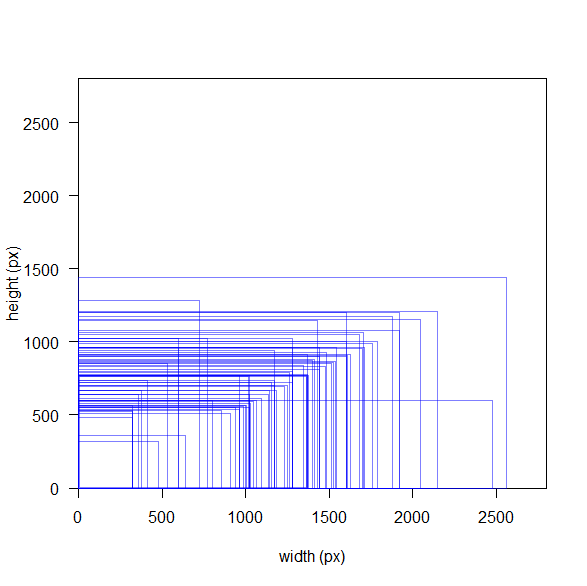
\includegraphics[height=\textheight]{images/devicesizes.png}
\end{center}
}

\frame{

\frametitle{{\normalsize Aside: Unique features of online studies}}

\begin{itemize}
\item<2-> Capacity for audio-visual treatments and measurements
\item<3-> Paradata collection
	\begin{itemize}
	\item Implicit outcomes like response times, answer switching, mouse click behavior, browser focus, eye tracking, etc.
	\end{itemize}
\item<4-> Complex randomization
\item<5-> Panel data
\item<5-> Synchronous, multi-person designs
\end{itemize}

}


\frame{

\frametitle{Non-textual Manipulations}

\small

\begin{itemize}\itemsep0.5em
\item Images can work well
\item Standalone or embedded in a text or question
\item<2-> Examples
	\begin{itemize}\footnotesize
	\item<2-> Kalmoe \& Gross\footnote{``Cueing Patriotism, Prejudice, and Partisanship in the Age of Obama: Experimental Tests of U.S. Flag Imagery Effects in Presidential Elections.'' \textit{Political Psychology}: in press.} measure impact of patriotic cues on candidate support by showing images of candidates with and without flags
	\item<3-> Subliminal primes possible, depending on software
	\item<4-> Lots of recent examples of facial manipulation
	\end{itemize}

\end{itemize}

}

\frame{

\frametitle{Example\footnote{Iyengar et al. 2010. ``Do Explicit Racial Cues Influence Candidate Preference? The Case of Skin Complexion in the 2008 Campaign.'' Working paper.}}

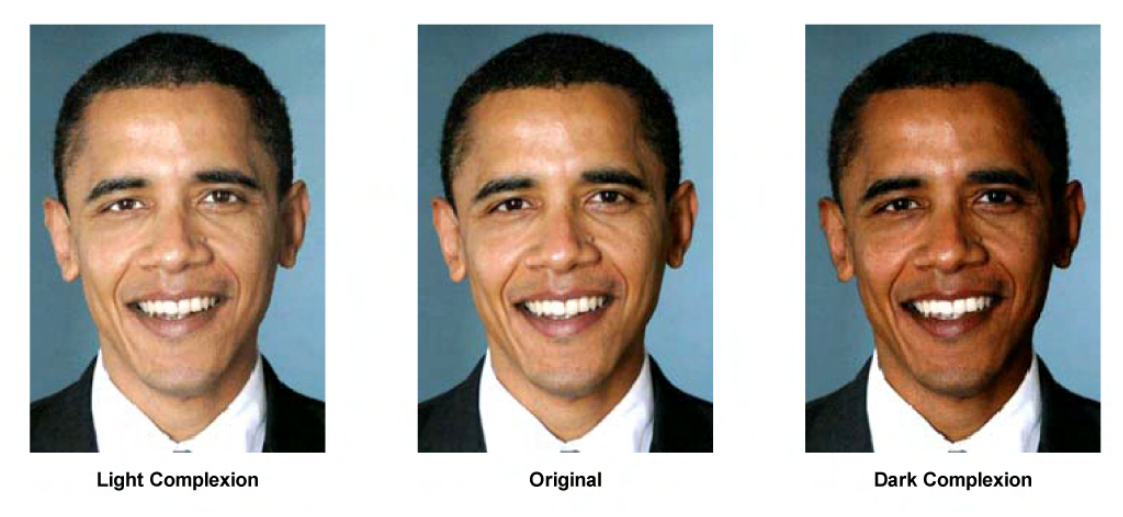
\includegraphics[width=\textwidth]{images/IyengarMessingBailenson}

}

\frame{

\frametitle{{\normalsize Example\footnote{Laustsen \& Petersen. 2016. ``Winning Faces vary by Ideology.'' \textit{Political Communication} 33(2): 188--211.}}}

\begin{center}
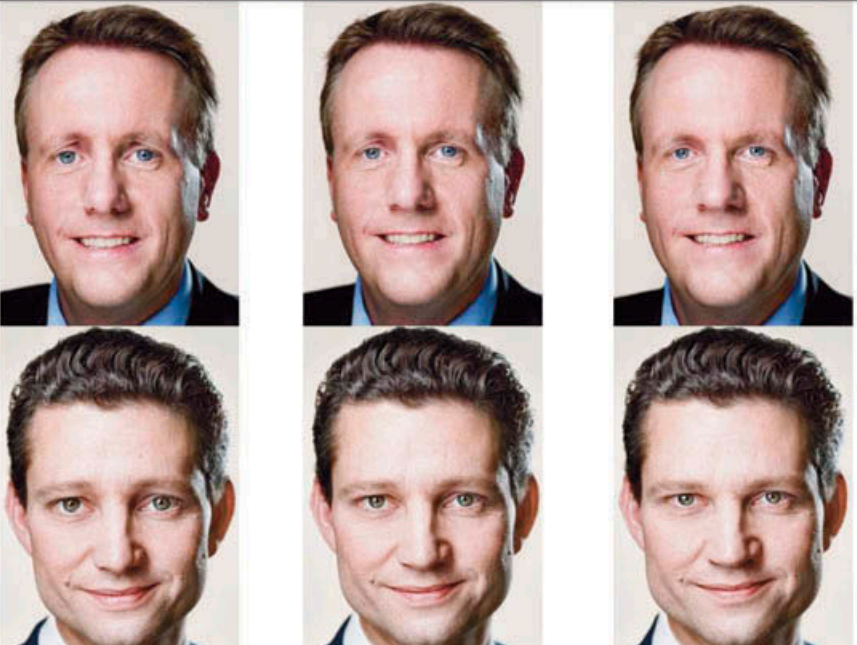
\includegraphics[width=\textwidth, trim={0cm 0cm 0cm 9cm}, clip]{images/laustsen}
\end{center}
}

\frame{
\frametitle{{\normalsize Example\footnote{Bailenson et al. 2006. ``Transformed Facial Similarity as a Political Cue: A Preliminary Investigation.'' \textit{Political Psychology} 27(3): 373--385.}}}

\begin{center}
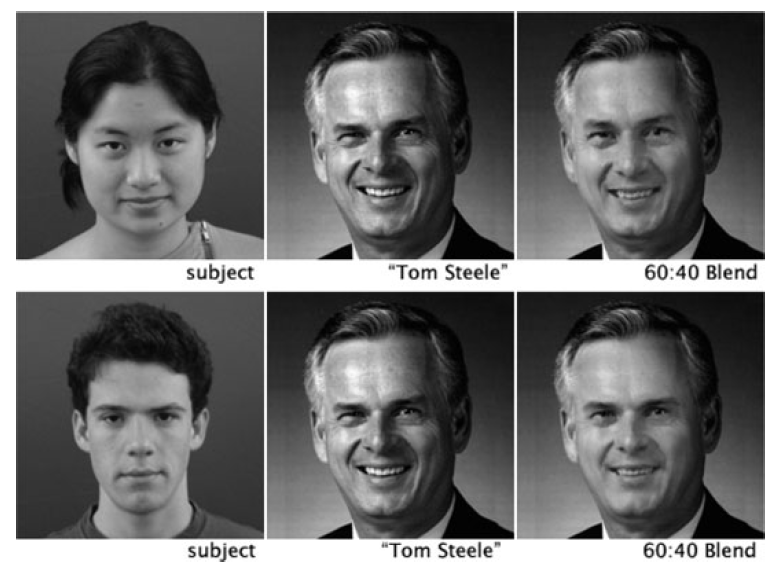
\includegraphics[width=\textwidth, trim={0cm 7.7cm 0cm 0cm}, clip]{images/BailensonGarlandIyengar}
\end{center}
}




\frame{

\frametitle{{\normalsize Audio \& Video manipulations}}

\small

\begin{itemize}\itemsep-0.2em
\item Problematic for same reasons as long texts
\item<2-> Best practices
	\begin{itemize}\footnotesize
	\item Keep it short
	\item Have the video play automatically
	\item Disallow survey progression
	\item Control and validate
	\end{itemize}
\item<3->Examples
	\begin{itemize}
	\item Television Advertisements\footnote{Vavreck. 2007 ``The Exaggerated Effects of Advertising on Turnout: The Dangers of Self-Reports.'' \textit{Quarterly Journal of Political Science} 2: 325--343.} 
	\item News Programs\footnote{Mutz. 2007. ``Effects of `In-Your-Face' Television Discourse on Perceptions of a Legitimate Opposition.'' \textit{American Political Science Review} 101(4): 621--635.}
	\end{itemize}	
\end{itemize}

}




\frame{
\frametitle{``Task'' Designs}

\begin{itemize}\itemsep0.5em
\item Task designs ask respondents to perform a task
\item Often developed for laboratory settings
\item<2-> Most common example: writing something
\item<3-> Can be problematic:
	\begin{itemize}
	\item Time-intensive
	\item Invites drop-off
	\item Compliance problems
	\end{itemize}
\end{itemize}

}


\againframe{ambivalentpartisan}



\questions


\frame{

\frametitle{Sensitive Item Designs}

\begin{itemize}
\item Experiments can also be used to measure something
\item Goal here is not necessarily causal inference, though the causal insight of the experiment provides \textit{descriptively} useful information
\item Paradigms
	\begin{itemize}
	\item List experiments
	\item Endorsement experiments
	\end{itemize}
\end{itemize}
}

\frame{

\frametitle{{\normalsize List Experiments \footnote{Kuklinski et al. 1997. ``Racial Prejudice and Attitudes Toward Affirmative Action.'' \textit{American Journal of Political Science} 41(2): 402--419.}}}

\small

Now I'm going to read you three things that sometimes make people angry or upset. After I read all three, just tell me \textit{how many} of them upset you. I don't want to know which ones. just \textit{how many}.

\footnotesize

\begin{enumerate}
\item the federal government increasing the tax on gasoline
\item professional athletes getting million-dollar salaries
\item large corporations polluting the environment
\item<2-> \textbf{a black family moving in next door}
\end{enumerate}


}

\frame{

\frametitle{{\normalsize Endorsement experiments\footnote{Lyall, Blair, \& Imai. 2013. ``Explaining Support for Combatants during Wartime: A Survey Experiment in Afghanistan.'' \textit{American Political Science Review} 107(4): 679--705.}}}

\small

A recent proposal \only<2>{\textbf{by the Taliban}} calls for the sweeping reform of the Afghan prison system, including the construction of new prisons in every district to help alleviate overcrowding in existing facilities. Though expensive, new programs for inmates would also be offered, and new judges and prosecutors would be trained. How do you feel about this proposal?
}




\questions


\StataActivity{Analysis of Example Experiments}











\frame{

\frametitle{Homework!}

\begin{itemize}
\item Get a sense of what can be studied survey-experimentally
\item Visit Time-Sharing Experiments for the Social Sciences
	\begin{itemize}
	\item \url{http://tessexperiments.org}
	\end{itemize}
\item Pick two studies from TESS
\item We will share them in tomorrow
\end{itemize}

}


\frame{}




\appendix


\section{Representativeness}
\frame{\tableofcontents[currentsection]}


\frame{
	\frametitle{Case selection}
	
	Our ambitions about what kind of inferences we want to derive from our descriptions influence how we select cases.
	
	
	\begin{itemize}\itemsep1em
	\item<2-> Purposive
	\item<3-> Comparative
	\item<4-> Representative
		\begin{itemize}
		\item<5-> Unrepresentative
		\end{itemize}
	\end{itemize}
}


\frame{
	\frametitle{Discuss in Pairs!}
	
	\Large
	\begin{center}
	What does it mean for a ``sample'' (set of cases) to be representative of a population?
	\end{center}
}

\frame{
	\frametitle{{\large Different conceptualizations}}
	
	\small
	
	\begin{itemize}\itemsep0.5em
		\item \textbf{Design-based}: A sample is representative because of how it was drawn (e.g., randomly)
		\item \textbf{Model-based}: A sample is representative because it resembles in the population with respect to certain variables (e.g., same proportion of women in sample and population, etc.)
		\item \textbf{Expert judgement}: A sample is representative as judged by an expert who deems it ``fit for purpose''
	\end{itemize}
}


\frame{
	\frametitle{Obtaining Representativeness}
	\begin{itemize}\itemsep0.5em
		\item<2-> Census
		\item<3-> Convenience/Purposive samples
		\item<4-> Quota sampling (common before 1940s)
		\item<5-> \textbf<7>{Simple random sampling}
		\item<6-> Complex survey designs
	\end{itemize}
}


\section{Design-based (Statistical) Sampling}
\frame{\tableofcontents[currentsection]}

\frame{
	\frametitle{{\normalsize Inference from Sample to Population}}
	\begin{itemize}\itemsep0.5em
	\item We want to know pop. parameter $\theta$
	\item We only observe sample estimate $\hat{\theta}$
	\item We have a guess but are also uncertain
	\vspace{1em}
	\item<2-> What range of values for $\theta$ does our $\hat{\theta}$ imply?
	\end{itemize}
}

\frame[label=srs]{
	\frametitle{Simple Random Sampling}
	\begin{enumerate}\itemsep0.5em
		\item Define target population
		\item Create ``sampling frame''
		\item Each unit in frame has equal probability of selection
		\item Collect data on each unit
		\item Calculate sample \textit{statistic}
		\item Draw an inference to the population
	\end{enumerate}
}


\begin{frame}[fragile]
\begin{center}
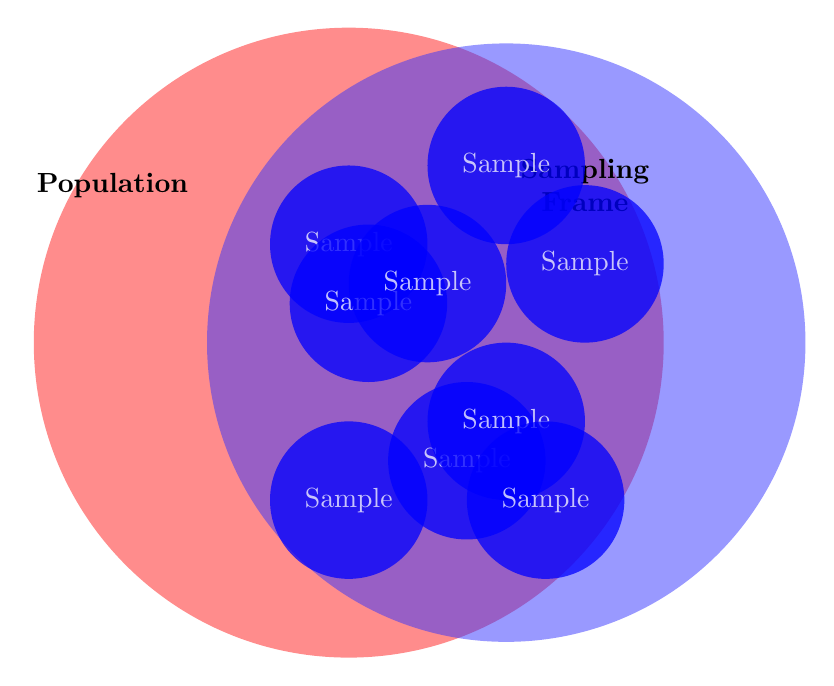
\begin{tikzpicture}
    \fill<1->[red!60,opacity=0.75] (0,0) circle (4cm) 
        node[text=white, align=center, text width=3cm] {};
    \node<1-> (pop) at (-3,2) {\textbf{Population}};
    \fill<2->[blue!80,opacity=0.5] (2,0) circle (3.8cm) 
        node[text=white, align=center, text width=3cm] {};
    \node<2->[align=center, text width=3cm] (pop) at (3,2) {\textbf{Sampling\\ Frame}};
    \fill<3->[blue,opacity=0.75] (1.5,-1.5) circle (1cm) 
        node[text=white, align=center, text width=3cm] {Sample};
    \fill<4->[blue,opacity=0.75] (3,1) circle (1cm) 
        node[text=white, align=center, text width=3cm] {Sample};
    \fill<4->[blue,opacity=0.75] (2,-1) circle (1cm) 
        node[text=white, align=center, text width=3cm] {Sample};
    \fill<4->[blue,opacity=0.75] (0,1.25) circle (1cm) 
        node[text=white, align=center, text width=3cm] {Sample};
    \fill<4->[blue,opacity=0.75] (.25,.5) circle (1cm) 
        node[text=white, align=center, text width=3cm] {Sample};
    \fill<4->[blue,opacity=0.75] (0,-2) circle (1cm) 
        node[text=white, align=center, text width=3cm] {Sample};
    \fill<4->[blue,opacity=0.75] (2,2.25) circle (1cm) 
        node[text=white, align=center, text width=3cm] {Sample};
    \fill<4->[blue,opacity=0.75] (1,.75) circle (1cm) 
        node[text=white, align=center, text width=3cm] {Sample};
    \fill<4->[blue,opacity=0.75] (2.5,-2) circle (1cm) 
        node[text=white, align=center, text width=3cm] {Sample};
\end{tikzpicture}
\end{center}
\end{frame}


\againframe{srs}

\frame{
	\frametitle{Statistical Inference I}

	To calculate a sample mean (or proportion):

	\begin{equation}
	\bar{y} = \frac{1}{n}\sum_{i=1}^{n}y_i
	\end{equation}
	{\small
	where $y_i = $ value for a unit, and\\
	$n = $ sample size
	}
	\vspace{0.5em}
	
	%This is a \textit{statistic} (the sample mean) that \textit{estimates} the population \textit{parameter} (the population mean)
	
}


\frame{
	\frametitle{Statistical Inference II}
	\begin{itemize}\itemsep1em
	\item If we calculate $\bar{y}$ in our \textit{sample}, what does this tell us about the $\bar{Y}$ in the \textit{population}?
	\item<2-> The sample \textit{estimate} is our guess at the value of the population \textit{parameter} within some degree of uncertainty
	\end{itemize}
}


\frame{
	\frametitle{Law of Large Numbers}
	\begin{itemize}
	\item Definition: The \textit{mean} of the $\hat{\theta}$ from each of a number of samples will converge on the population $\theta$, as the number of samples increases
	\end{itemize}
}

\frame{
	\frametitle{Sampling Variance}
	\begin{itemize}\itemsep1em
	\item The $\hat{\theta}$ in any particular sample can differ from the population value $\theta$
	\item This variation is calling ``sampling variance'' or ``sampling error''
	\item The standard error describes the average amount of variation of the $\hat{\theta}$'s around $\theta$
\end{itemize}
}


\frame{
	\frametitle{How Uncertain Are We?}
	\begin{itemize}\itemsep1em
	\item Our uncertainty depends on sampling procedures
	\item Most importantly, \textit{sample size}
		\begin{itemize}
		\item As $n \rightarrow \infty$, uncertainty $\rightarrow 0$
		\end{itemize}
	\item We typically summarize our uncertainty as the \textit{standard error}
	\end{itemize}
}

\frame{
	\frametitle{Standard Errors (SEs)}
	\begin{itemize}\itemsep1em
	\item Definition: ``The standard error of a sample estimate is the average distance that a sample estimate ($\hat{\theta}$) would be from the population parameter ($\theta$) if we drew many separate random samples and applied our estimator to each.''
	\item<2-> Square root of the sampling variance
\end{itemize}
}


\frame{
	\frametitle{Sample mean}
	
	\small
	
	\begin{equation}
	\bar{y} = \frac{1}{n}\sum_{i=1}^{n}y_i
	\end{equation}
	where $y_i = $ value for a unit, and\\
	$n = $ sample size
	
	\begin{equation}
	SE_{\bar{y}} = \sqrt{(1-f)\frac{s^2}{n}}
	\end{equation}
	where $f = $ proportion of population sampled,\\
	$s^2 = $ sample (element) variance, and\\
	$n = $ sample size
}

\frame{
	\frametitle{SATE}
	
	\small
	
	\begin{equation}
	\hat{SATE} = \frac{1}{n_1}\sum_{i=1}^{n_1}y_{i,1} - \frac{1}{n_0}\sum_{i=1}^{n_1}y_{i,0}
	\end{equation}
	where $y_{i,1} = $ value for a treatment group unit, and\\
	$y_{i,0} = $ value for a control group unit, and\\
	$n_1, n_0 = $ group sample sizes
	
	
	\begin{equation}
	\widehat{Var}(SATE) = \dfrac{\widehat{Var}(y_1)}{n_1} + \dfrac{\widehat{Var}(y_0)}{n_0}
	\end{equation}
	where $Var(y_0) = \sum_{i=1}^{n_0}(y_{i,0} - \bar{y}_0)^2$,\\
	$Var(y_1) = \sum_{i=1}^{n_1}(y_{i,1} - \bar{y}_1)^2$, and\\
	$n_1, n_0 = $ group sample sizes
}

\questions


\frame{}


\section{Response Rates}
\frame{\tableofcontents[currentsection]}

\frame{
    \frametitle{Response Rates}
    \begin{itemize}\itemsep1em
        \item Why do we care?
        \item<2-> Survey Error
            \begin{itemize}
                \item<2-> Variance
                \item<2-> Bias
            \end{itemize}
        \item<3-> Sample size calculations (and design effects) are based on completed interviews
        \item<4-> Cost, time, and effort
    \end{itemize}
}

\frame{
    \frametitle{Response Rates}
    \begin{itemize}
        \item Imagine we need $n=1000$
        \item How many attempts to obtain that sample:\\
        \vspace{1em}
        \begin{tabular}{l r}\toprule
        Response Rate & Needed Attempts\\ \midrule
        1.00 & 1000 \\
        0.75 & 1333 \\
        0.50 & 2000 \\
        0.25 & 4000 \\
        0.10 & 10,000 \\ \bottomrule
        \end{tabular}
    \end{itemize}
}


\frame{
	\frametitle{Response Rate}
	\begin{itemize}\itemsep1em
		\item Interviews divided by eligibles
		\item $RR = \frac{I}{E}$
		\item Challenges
    		\begin{itemize}
        		\item Unknown eligibility
        		\item Partial interviews
        		\item Non-probability samples
        		\item Complex survey designs
    		\end{itemize}
        \item Cooperation Rate (I's divided by contacts)
	\end{itemize}
}

\frame<1>[label=codes]{
	\frametitle{Disposition Codes}
	\begin{itemize}\itemsep1em
		\item Complete Interview (I)
		\item Partial Interview (P)
		\item Non-interviews
    		\begin{itemize}
        		\item Refusal (R)
        		\item Non-contact (NC)
        		\item Other (O)
    		\end{itemize}
		\item<2> Unknowns (U)
		\item<2> Ineligibles
	\end{itemize}
}

\frame{
	\frametitle{What is a refusal?}
	\begin{itemize}\itemsep2em
		\item<1-> How do categorize a respondent as a refusal?
		\item<2-> When can we try to convert an apparent refusal?
	\end{itemize}
}


\frame{
	\frametitle{What is a refusal?}
	\begin{itemize}\itemsep1em
		\item<1-> ``I don't want to participate.''
		\item<2-> ``I'm too busy to do this right now.''
		\item<3-> ``What do I get for my time?''
		\item<4-> (Hang-up phone without saying anything.)
		\item<5-> ``Okay, but I only have 5 minutes.''
		\item<6-> ``My husband can do it if you call back.''
		\item<7-> ``How did you get my number?''
		\item<8-> ``Go f' yourself.''
	\end{itemize}
}


\againframe{codes}

\frame{
	\frametitle{Eligibility}
	\begin{itemize}\itemsep2em
		\item<1-> Why would an ineligible unit be in our sample?
		\item<2-> How do we determine ineligibility?
		\item<3-> What do we do with ``unknowns''?
	\end{itemize}
}


\frame{
	\frametitle{Response Rate 1\footnote{Note: Simplified slightly}}
	\Large
	\begin{itemize}\itemsep2em
		\item $RR1 = \frac{I}{(I + P) + (R + NC) + U}$
	\end{itemize}
}

\frame{
	\frametitle{Response Rate 2\footnote{Note: Simplified slightly}}
    \Large
	\begin{itemize}\itemsep2em
		\item $RR2 = \frac{I + P}{(I + P) + (R + NC) + U}$
	\end{itemize}
}

\frame{
	\frametitle{Response Rates 3 and 4\footnote{Note: Simplified slightly}}
	\Large
    \begin{itemize}\itemsep2em
		\item $RR3 = \frac{I}{(I + P) + (R + NC) + (e*U)}$
		\item $RR4 = \frac{I + P}{(I + P) + (R + NC) + (e*U)}$
		\vspace{1em}
		\item $e$ is estimated proportion eligible among unknowns
	\end{itemize}
}

\frame{
	\frametitle{Refusal Rates}
	\begin{itemize}\itemsep2em
		\item Related to response rate
		\item Numerator is refusals
		\item E.g., {\Large $REF1 = \frac{R}{(I + P) + (R + NC) + U}$}
	\end{itemize}
}

\frame{
	\frametitle{Complex Survey Designs}
	\begin{itemize}\itemsep2em
		\item Stratified Sampling (unequal allocation)
    		\begin{itemize}
        		\item Sums of codes weighted by $\frac{1}{p}$
        		\item $p$ is probability of selection
        		\item May want to report stratum-specific rates
    		\end{itemize}
    	\item Multi-stage sampling (e.g., cluster sampling)
        	\begin{itemize}
            	\item RR is product of cluster cooperation and within-cluster response rate
        	\end{itemize}
	\end{itemize}
}


\frame{
	\frametitle{Internet Surveys}
	\begin{itemize}\itemsep2em
		\item For \textit{probability-based samples}, RR is a product of:
    		\begin{itemize}
        		\item Recruitment Rate (RR for panel enrollment)
        		\item Completion Rate (RR for specific survey)
        		\item Profile Rate (in some cases)
        		\item E.g., if Recruitment Rate is 30\% and Completion Rate is 80\%, $RR = 0.3 * 0.8 =$ 24\%
    		\end{itemize}
    	\item For \textit{non-probability samples}, RR is undefined
        	\begin{itemize}
            	\item No sampling involved (so no denominator)
            	\item If from panel, report Completion Rate
            	\item If fully opt-in, there's nothing you can do
        	\end{itemize}
	\end{itemize}
}


\frame{
\frametitle{Differential Response Rates}
\begin{itemize}\itemsep2em
\item Experimental inference breaks if treatment causes breakoff or item nonresponse
\item If known in advance, you should:
	\begin{itemize}
		\item Change the experiment
		\item Differential incentives
		\item Mode differences
	\end{itemize}
\item If discovered in field, you can:
	\begin{itemize}
		\item Add/modify incentives
		\item Refusal conversion
	\end{itemize}
\end{itemize}
}



\section{Regression Analysis}
\frame{\tableofcontents[currentsection]}


\frame{
	\frametitle{Uses of Regression}
	\begin{enumerate}\itemsep2em
	\item Description
	\item Prediction
	\item Causal Inference
	\end{enumerate}
}

\frame{
	\frametitle{Descriptive Inference}
	\begin{enumerate}\itemsep1em
	\item We want to understand a \textit{population} of cases
	\item We cannot observe them all, so:
		\begin{enumerate}
    		\item Draw a \textit{representative} sample
    		\item Perform mathematical procedures on sample data
    		\item Use assumptions to make inferences about population
    		\item Express uncertainty about those inferences based on assumptions
		\end{enumerate}
	\end{enumerate}
}

\frame{
	\frametitle{Parameter Estimation}
	\begin{itemize}\itemsep1em
    	\item We want to observe population \textit{parameter} $\theta$
    	\item If we obtain a representative sample of population units:\\
    		\begin{itemize}\itemsep1em
        		\item Our sample statistic $\hat{\theta}$ is an unbiased estimate of $\theta$
        		\item Our sampling procedure dictates how uncertain we are about the value of $\theta$
    		\end{itemize}
	\end{itemize}
}


\frame{
	\frametitle{Causal Inference}
	\begin{enumerate}\itemsep1em
	\item<2-> Everything that goes into descriptive inference
	\item<3-> Plus, philosophical assumptions
	\item<4-> Plus, randomization \textit{or} perfectly specified model
	\end{enumerate}
}



\subsection{OLS}
\frame{\tableofcontents[currentsection]}


\frame{
\frametitle{Relationship}

\begin{itemize}\itemsep1em
\item<1-> Covariance:\\
	$Cov(X,Y) = \sum_{i=1}^{n} \dfrac{(X_i - \bar{X})(Y_i - \bar{Y})}{n-1}$
\item<2-> Pearson's Correlation:\\
	{\small $Corr(X,Y) = r_{x,y} = \sum_{i=1}^{n} \dfrac{(X_i - \bar{X})(Y_i - \bar{Y})}{(n-1)s_x s_y}$}
\end{itemize}
}


\frame{

\frametitle{Correlation is linear!}

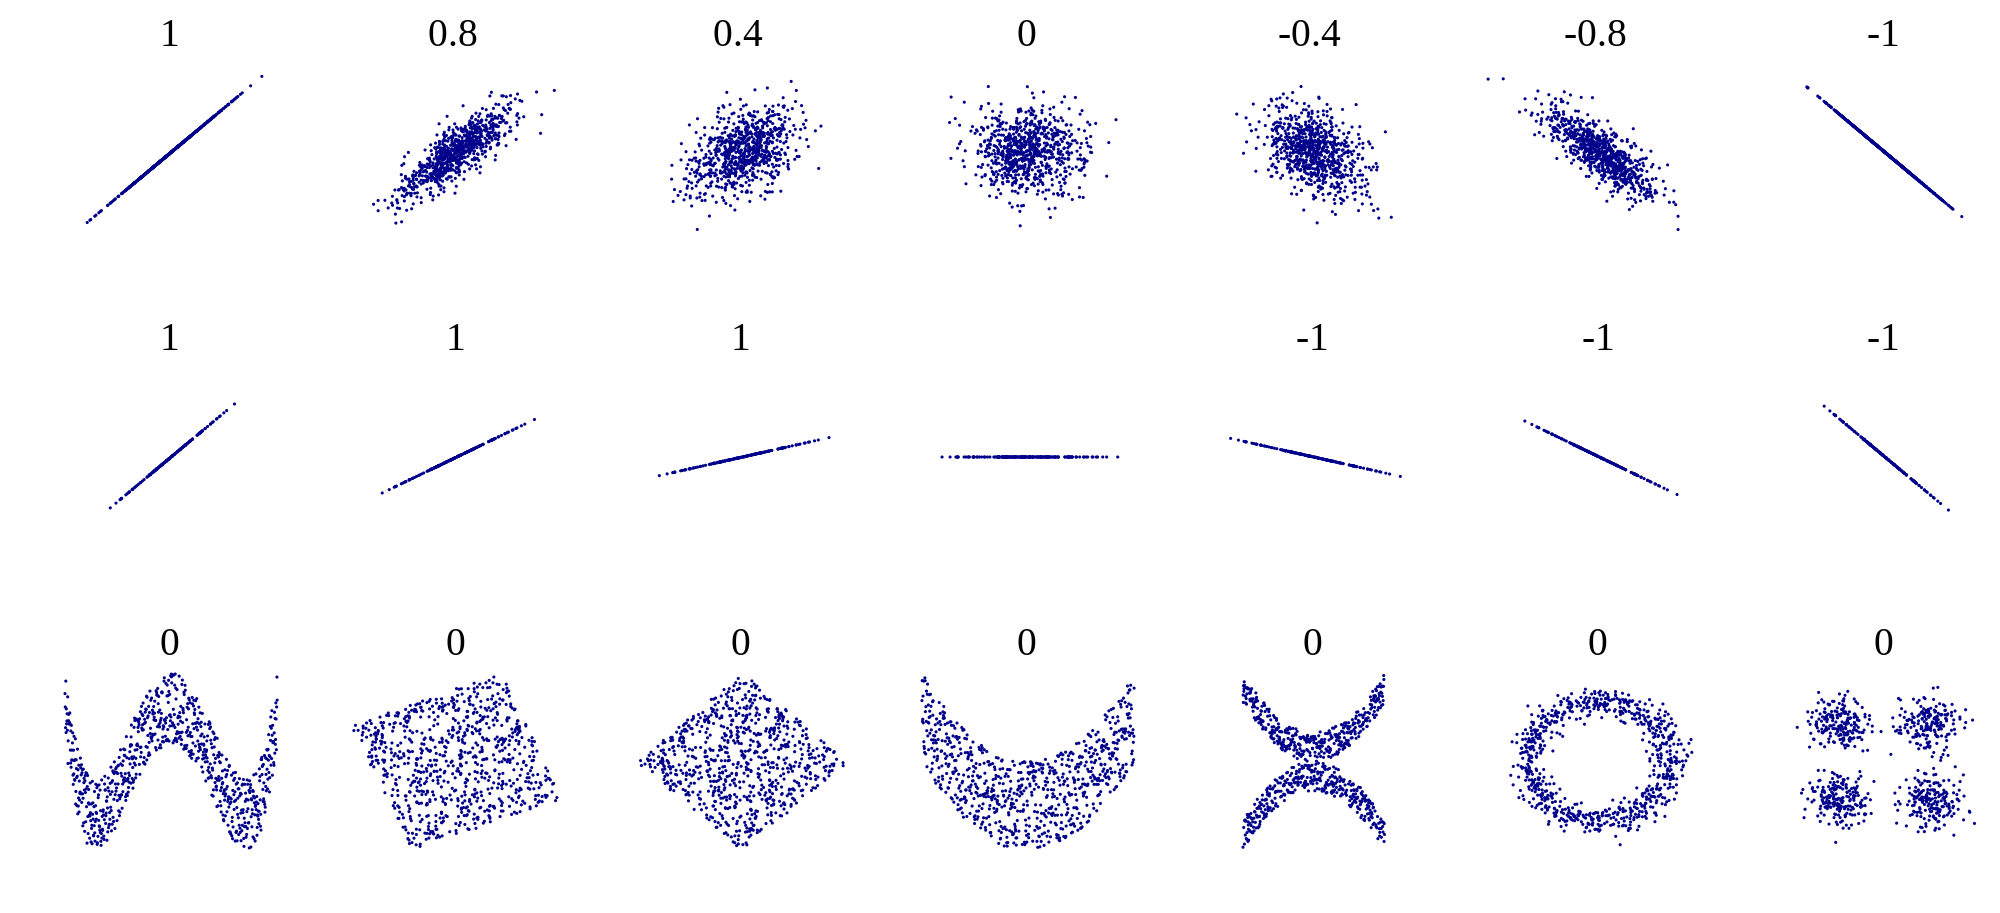
\includegraphics[width=\textwidth]{images/correlation}

\vspace{1em}
{\footnotesize Source: \href{https://commons.wikimedia.org/wiki/File:Correlation_examples2.svg}{Wikimedia}}
}


\frame{

	\frametitle{Analyzing Complex Surveys}
	
	\small
	
	\begin{itemize}\itemsep1em
	\item There's a saying: ``Every simple random survey is simple in the same way, but every complex survey is complex in its own way.''
	\item<2-> Statistics courses will almost always assume simple random sampling
	\item<3-> Any sample that is not self-weighting requires more complicated \textit{estimators} that account for varying weights
	\item<4-> Don't try to do this by hand
		\begin{itemize}
 		\item \href{http://www.stata.com/manuals13/svy.pdf}{Stata \texttt{svy} module}
 		\item \href{https://cran.r-project.org/web/packages/survey/index.html}{R \texttt{survey} package}
		\end{itemize}
	\end{itemize}

}


\frame<1-5,2>[label=ways]{
	\frametitle{Ways of Thinking About OLS}
	\begin{enumerate}\itemsep1em
    	\item<2-> Estimating Unit-level Causal Effect
    	\item<3-> Ratio of $Cov(X,Y)$ and $Var(X)$
    	\item<4-> Minimizing residual sum of squares (SSR)
    	\item<5-> Line (or surface) of best fit
	\end{enumerate}
}


\frame{
	\frametitle{Bivariate Regression I}
	\begin{itemize}\itemsep1em
	\item $Y$ is continuous
	\item $X$ is a randomized treatment indicator/dummy $(0,1)$
	\item How do we know if the treatment $X$ had an effect on $Y$?
	\item<2-> Look at mean-difference: $E[Y_i|X_i=1] - E[Y_i|X_i=0]$
	\end{itemize}
}


\frame{
	\frametitle{Three Equations}
	\begin{enumerate}\itemsep2em
	\item Population: $Y = \beta_0 + \beta_1 X \hspace{0.5em} (+ \epsilon)$
	\item Sample estimate: $\hat{y} = \hat{\beta}_0 + \hat{\beta}_1 x$
	\item Unit:
		\begin{align*}
		y_i & = \hat{\beta}_0 + \hat{\beta}_1 x_i + e_i\\
		    & = \bar{y}_{0i} + (y_{1i} - y_{0i}) x_i + (y_{0i} - \bar{y}_{0i})
		\end{align*}
	\end{enumerate}
}


\frame<1-2>[label=dummy]{
	\frametitle{Bivariate Regression I}
	\begin{itemize}\itemsep1em
    	\item Mean difference ($E[Y_i|X_i=1] - E[Y_i|X_i=0]$) is the regression line slope
    	\item Slope ($\beta$) defined as $\frac{\Delta Y}{\Delta X}$
    		\vspace{1em}
    		\begin{itemize}\itemsep1em
        		\item<2-> $\Delta Y = E[Y_i|X=1] - E[Y_i|X=0]$
        		\item<2-> $\Delta X = 1 - 0 = 1$
    		\end{itemize}
    	\item<3-> How do we know if this is a \textit{significant} difference?
    		\begin{itemize}
        		\item We'll come back to that
    		\end{itemize}
	\end{itemize}

}

% graphs of mean-difference
% http://thomasleeper.com/regcourse/Slides-2014/Session02_01.html#20


\frame[label=bivariate1]{
	\begin{center}
	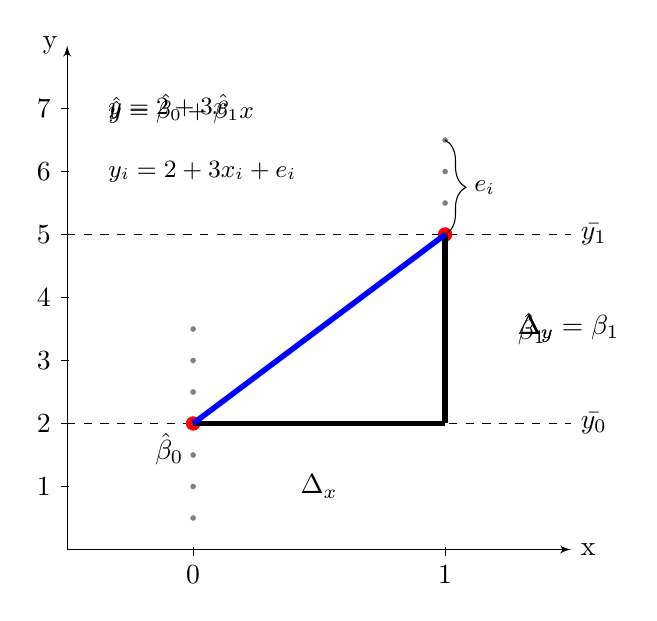
\begin{tikzpicture}[>=latex', scale=0.8]
        \draw[->] (0,0) node[below] (origin) {}  -- (8,0) node[right] (xaxis) {x};
        \draw[->] (origin) -- (0,8) node[left] (yaxis) {y};
        % x ticks
        \draw (2,1pt) -- (2,-3pt) node[anchor=north] {0};
        \draw (6,1pt) -- (6,-3pt) node[anchor=north] {1};
        % y ticks
        \foreach \y in {1,...,7}
             \draw (1pt,\y) -- (-3pt,\y) node[anchor=east] {$\y$};
        
        % points
        \foreach \y in {0.5,1.0,...,3.5} {
        	\draw[gray,fill] (2,\y) circle [radius=1pt];
        	\draw[gray,fill] (6,3+\y) circle [radius=1pt];
        }
        % y_0-bar
        \draw<2-4>[dashed] (0,2) -- (8,2) node[right] {$\bar{y_0}$};
        % y_1-bar
        \draw<2-4>[dashed] (0,5) -- (8,5) node[right] {$\bar{y_1}$};
        % mean points
        \draw<2->[red,fill] (2,2) circle [radius=3pt];
        \draw<2->[red,fill] (6,5) circle [radius=3pt];
        
        % slope
        \draw<3-4>[solid, line width=2pt] (2,2) -- (6,2);
        \draw<3-5>[solid, line width=2pt] (6,2) -- (6,5);
        \node<3-4>(deltax) at (4,1) {$\Delta_x$};
        \node<3>[right](deltay) at (7,3.5) {$\Delta_y$};
        \node<4>[right](deltay) at (7,3.5) {$\Delta_y = \beta_1$};
        \node<5>[right](deltay) at (7,3.5) {$\hat{\beta}_1$};
        
        \draw<4->[blue, solid, line width=2pt] (2,2) -- (6,5);
        \node<4-5>[below left](b0) at (2,2) {$\hat{\beta}_0$};
        
        \node<5>[right](eq) at (0.5,7) {\small $\hat{y} = \hat{\beta}_0 + \hat{\beta}_1 x$};
        \node<6->[right](eq) at (0.5,7) {\small $\hat{y} = 2 + 3 x$};
        \node<7->[right](eq) at (0.5,6) {\small $y_i = 2 + 3 x_i + e_i$};
        \draw<7->[right,decorate,decoration={brace,mirror,amplitude=7.5pt}] (6,5)  -- (6,6.5)
        	node [right, pos=0.5, xshift=7] {\small $e_i$};
    \end{tikzpicture}
    \end{center}
}

% OLS only makes sense in a linear world

\frame{
	\frametitle{Systematic versus unsystematic component of the data}
	\begin{itemize}\itemsep1em
    	\item Systematic: Regression line (slope)
    		\begin{itemize}
    		\item Linear regression estimates the conditional means of the population data (i.e., $E[Y|X]$)
    		\end{itemize}
    	\item Unsystematic: Error term is the deviation of observations from the line
    		\begin{itemize}
        		\item The difference between each value $y_i$ and $\hat{y}_i$ is the \textit{residual}: $e_i$
        		\item OLS produces an estimate of the relationship between X and Y that minimizes the \textit{residual sum of squares}
    		\end{itemize}
	\end{itemize}
}

\frame{
	\frametitle{Why are there residuals?}
	\begin{itemize}\itemsep1em
		\item<2-> Omitted variables
		\item<2-> Measurement error
		\item<2-> Fundamental randomness
	\end{itemize}
}


\frame{}


\section{Opinion Questions}
\frame{\tableofcontents[currentsection]}


\frame{
	\frametitle{Evaluative questions}
	\begin{itemize}\itemsep1em
		\item Name an object of evaluation
		\item Possibly describe that object
		\item Ask for a transformation of the evaluation onto a set of responses
	\end{itemize}
}

\frame{
	\frametitle{Question templates}

	\small
	
	\begin{itemize}
		\item Ratings
			\begin{itemize}
				\item Several varieties of rating scales
			\end{itemize}
		\item Scales/Thermometers
		\item Agree-disagree
		\item Forced choices
		\item Open-ended
		\item Rankings (note: need alternatives to rank against)
	\end{itemize}
}

\frame{
	\frametitle{Extended Example}
	\begin{itemize}\itemsep1em
		\item Public opinion survey in Great Britain
		\item Construct: Opinion toward UK involvement in air strikes on Islamic State militants in Iraq and Syria
		\item Think about strengths and weaknesses of each question
	\end{itemize}
}

\frame{
	\frametitle{{\large Example: Rating (bipolar)}}
	Do you support or oppose Great Britain's participation in U.S.-led air strikes on Islamic State (IS) in Iraq and Syria?
	\begin{itemize}
		\item Strongly support
		\item Somewhat support
		\item Neither support nor oppose
		\item Somewhat oppose
		\item Strongly oppose
	\end{itemize}
}

\frame{
	\frametitle{{\large Example: Rating (branching)}}
	
	\footnotesize
	
	Do you support or oppose Great Britain's participation in U.S.-led air strikes on Islamic State (IS) in Iraq and Syria?
	\begin{itemize}
		\item Support
		\item Neither support nor oppose
		\item Oppose
	\end{itemize}
	\vspace{1em}
	Would you say that you strongly [support|oppose] or somewhat [support|oppose] Great Britain's participation?
	\begin{itemize}
		\item Strongly
		\item Somewhat
	\end{itemize}
}

\frame{
	\frametitle{{\large Example: Rating (bipolar)}}
	Are you favourable or unfavourable toward Great Britain's participation in U.S.-led air strikes on Islamic State (IS) in Iraq and Syria?
	\begin{itemize}
		\item Very favourable
		\item Somewhat favourable
		\item Neither favourable nor unfavourable
		\item Somewhat unfavourable
		\item Strongly unfavourable
	\end{itemize}
}

\frame{
	\frametitle{{\large Example: Rating (unipolar)}}
	To what extent do you support Great Britain's participation in U.S.-led air strikes on Islamic State (IS) in Iraq and Syria?
	\begin{itemize}
		\item Strongly
		\item Moderately
		\item Somewhat
		\item Not at all
	\end{itemize}
}

\frame{
	\frametitle{{\large Example: Rating (unipolar)}}
	How favourable are you toward Great Britain's participation in U.S.-led air strikes on Islamic State (IS) in Iraq and Syria?
	\begin{itemize}
		\item Extremely favourable
		\item Very favourable
		\item Moderately favourable
		\item Somewhat favourable
		\item Not at all favourable
	\end{itemize}
}

\frame{
	\frametitle{{\large Example: Numbered Scale}}
	
	\small
	
	On a scale from 1 to 5, with 1 being ``strongly oppose'' and 5 being ``strongly support,'' to what extent do you support Great Britain's participation in U.S.-led air strikes on Islamic State (IS) in Iraq and Syria?
	\begin{enumerate}
		\item Strongly oppose
		\item 
		\item 
		\item 
		\item Strongly support
	\end{enumerate}
}

\frame{
	\frametitle{{\large Example: Thermometer}}
	
	\footnotesize
	
	We would like to get your feelings toward some of political policies. Please rate your support for the policy using something we call the feeling thermometer. Ratings between 50 degrees and 100 degrees mean that you feel favourable and warm toward the policy. Ratings between 0 degrees and 50 degrees mean that you don't feel favourable toward the policy. You would rate the policy at the 50 degree mark if you don't feel particularly favourable or unfavourable toward.
	
	\vspace{1em}
	Great Britain's participation in U.S.-led air strikes on Islamic State (IS) in Iraq and Syria.
	\begin{itemize}
		\item 0--100 slider
	\end{itemize}
}


\frame{
	\frametitle{{\normalsize Example: Agree/Disagree (bipolar)}}
	To what extent do you agree with the following statement: I support Great Britain's participation in U.S.-led air strikes on Islamic State (IS) in Iraq and Syria.
	\begin{itemize}
		\item Strongly agree
		\item Somewhat agree
		\item Neither agree nor disagree
		\item Somewhat disagree
		\item Strongly disagree
	\end{itemize}
}

\frame{
	\frametitle{{\normalsize Example: Agree/Disagree (unipolar)}}
	To what extent do you agree with the following statement: I support Great Britain's participation in U.S.-led air strikes on Islamic State (IS) in Iraq and Syria.
	\begin{itemize}
		\item Agree completely
		\item Agree to a large extent
		\item Agree to a moderate extent
		\item Agree a little bit
		\item Agree not at all
	\end{itemize}
}

\frame{
	\frametitle{{\large Example: Forced choice}}
	When thinking about Great Britain's participation in U.S.-led air strikes on Islamic State (IS) in Iraq and Syria, which of the following comes closer to your opinion:
	\begin{itemize}
		\item Great Britain should participate in air strikes
		\item Great Britain should not participate in air strikes
	\end{itemize}
}

\frame{
	\frametitle{{\large Example: Open-ended}}
	In your own words, how would you describe your opinion on Great Britain's participation in U.S.-led air strikes on Islamic State (IS) in Iraq and Syria?
}


\frame{
	\frametitle{Additional Considerations}
	\begin{itemize}\itemsep0.5em
		\item How many response categories?
		\item Middle category (presence and label)
		\item ``no opinion'' and/or ``don't know'' options
		\item Probe if ``no opinion'' or ``don't know''?
		    \begin{itemize}
                \item Encourage guessing?
    		    \item Clarify/describe object of evaluation?
		    \end{itemize}
		\item Branching format?
		\item Order of response categories
		\item Changes based on survey mode
	\end{itemize}
}





\section{Research Ethics}
\frame{\tableofcontents[currentsection]}

\frame{
\frametitle{History: Key Moments}

\small

\begin{enumerate}
\item Tuskegee (1932-1972) and Guatemala (1946-1948) Studies
\item Nuremberg Code (1947)
\item Helsinki Declaration (1964)
\item U.S. 45 CFR 46 (1974) and ``Common Rule'' (1991)
\item The Belmont Report (1979)
\item EU Data Protection Directive (1995; 2012)
	\begin{itemize}
	\item UK Data Protection Act (1998)
	\end{itemize}
\end{enumerate}
}


\frame{
	\frametitle{Helsinki Declaration}
	
	\small
	\begin{itemize}
	\item Adopted by the World Medical Association in 1964\footnote{\url{http://www.bmj.com/content/2/5402/177}}
	\item Narrowly focused on medical research
	\item Expanded the Nuremberg Code
		\begin{itemize}
		\item Relaxed consent requirements
		\item Risks should not exceed benefits
		\item Institutionalization of ethics oversight
		\end{itemize}
	\item<2-> Do these rules apply to non-medical research?
	\end{itemize}

}

\frame{
	\frametitle{The Belmont Report}
	
	\small
	\begin{itemize}
	\item Commissioned by the U.S. Government in 1979\footnote{\url{http://www.hhs.gov/ohrp/humansubjects/guidance/belmont.html}}
	\item Three overarching principles:
		\begin{enumerate}
		\item Respect for persons
		\item Beneficence
		\item Justice
		\end{enumerate}
	\item Three policy implications:
		\begin{itemize}
		\item Informed consent
		\item Assessment of risks/benefits
		\item Care for vulnerable populations
		\end{itemize}
	\end{itemize}

}

\frame{
\frametitle{Benefits and Harm}
	\begin{itemize}\itemsep1em
	\item What is a ``benefit''?
	\item What is a ``harm''?
	\item How do we balance the two?
	\end{itemize}
}


\frame{

\frametitle{Ethical Considerations}

\begin{itemize}
\item Most ethical issues are not unique to \textit{experimental} social science
\item Some especially important issues:
	\begin{enumerate}
	\item Randomization
	\item Informed consent
	\item Privacy
	\item Deception
	\item Publication bias
	\end{enumerate}
\end{itemize}

}

\frame{

\frametitle{I. Randomization}

\begin{itemize}
\item Is it ethical to randomize?
\end{itemize}

}



\frame{
	\frametitle{II. Informed Consent}
	\begin{itemize}
	\item Persons must consent to being a research subject
	\item<2-> What this means in practice is complicated
		\begin{itemize}
		\item What is consent?
		\item What is ``informed'' consent?
		\item What exactly do they have to consent to?
		\end{itemize}
	\item<3-> Cross-national variations
		\begin{itemize}
		\item Consent forms required in U.S.
		\item Not required in UK
		\end{itemize}
	\end{itemize}

}


\frame{
	\frametitle{III. Privacy}
	\begin{itemize}\itemsep0.5em
	\item Under EU Data Protection Directive (1995), data can be processed when:
		\begin{itemize}
		\item Consent is given
		\item Data are used for a ``legitimate'' purpose
		\item Anonymous or confidential
		\end{itemize}
	\item Data cannot leave the EU except under conditions
	\end{itemize}

}

\frame{
	\frametitle{III. Privacy}
	\begin{itemize}\itemsep1em
	\item Experimental might be additionally sensitive
	\item<2-> Answers reflect ``manipulated'' attitudes, behaviors, perceptions, etc. that respondents may not have given in another setting
	\end{itemize}

}



\frame{

\frametitle{IV. Deception}

\begin{itemize}
\item Major distinction between psychology tradition and economics tradition\footnote{Dickson, E. 2011. ``Economics versus Psychology Experiments.'' \textit{Cambridge Handbook of Experimental Political Science}.}
	\begin{itemize}
	\item Purpose of the study
	\item Purpose of specific items or tasks
	\item Order or length of questionnaire
	\end{itemize}
\item<2-> Psychologists focus on \textit{debriefing}
\item<3-> Within economics, norms about \textit{acts of omission} versus \textit{acts of commission}
	\begin{itemize}
	\item<4-> Omission: In a multi-round trust game, an additional round is added
	\item<5-> Commission: Telling respondents it is a dictator game, but it is actually a trust game
	\end{itemize}
\end{itemize}


}


\frame{

\frametitle{V. Publication Bias}

\begin{itemize}\itemsep0.5em
\item Publication bias not typically discussed as an ethical question
\item<2-> If studies are meant to policy or practical implications, then we care about PATE or a set of CATEs, including whether their effects are positive, negative, or zero.
\item<3-> Publication bias (toward ``significant'' results) invites wasting resources on treatments that actually don't work
\end{itemize}

}



\frame{
	\frametitle{{\normalsize Lots of Other Ethical Questions}}
	\begin{enumerate}
	\item<2-> Funding
	\item<3-> Independence and Politicization
	\item<4-> Vulnerable populations (e.g. children, sick)
	\item<5-> Incentives
	\item<6-> Cross-national research
	\item<7-> End uses/users of research
	\item<8-> Others\dots
	\end{enumerate}
}

\questions



\end{document}
